\documentclass{beamer}

%% \documentclass[handout]{beamer}
%% % use this with the [handout] option to create handouts for the audience
%% \usepackage{pgfpages}
%% \pgfpagesuselayout{2 on 1}[a4paper,border shrink=5mm]

\mode<presentation>
{
  \usetheme{Diku}
% set this to your preferences:
%  \setbeamercovered{invisible}
  \setbeamercovered{transparent}
}

\usepackage{graphicx}
\usepackage{epic}

\usepackage{amsmath}
\usepackage{amssymb}
\usepackage{amsthm}

\usepackage{minibox}
\usepackage{listings}
\newcommand{\basetop}[1]{\vtop{\vskip-1ex\hbox{#1}}}
\newcommand{\source}[1]{\let\thefootnote\relax\footnotetext{\scriptsize\textcolor{kugray1}{Source: #1}}}

% for coloured code citation in text:
\usepackage{fancyvrb}

%%%%%%%%%%%%%%%%%%%%%%%%%%%%%%%%%
%%%%%    code sections   %%%%%%%%
%%%%%%%%%%%%%%%%%%%%%%%%%%%%%%%%%

% code highlighting commands in own block
\DefineVerbatimEnvironment{code}{Verbatim}{fontsize=\scriptsize}
\DefineVerbatimEnvironment{icode}{Verbatim}{fontsize=\scriptsize}

% Fancy code with color commands:
\DefineVerbatimEnvironment{colorcode}%
        {Verbatim}{fontsize=\scriptsize,commandchars=\\\{\}}

%%%%%%%%%%%%%%%%%%%%%%%%%%%%%%%%%%
%%%%%    some coloring    %%%%%%%%

\definecolor{Red}{RGB}{220,50,10}
\definecolor{Blue}{RGB}{0,51,102}
\definecolor{Yellow}{RGB}{102,51,0}
\definecolor{Orange}{RGB}{178,36,36}
\definecolor{Grey}{RGB}{180,180,180}
\definecolor{Green}{RGB}{20,120,20}
\definecolor{Purple}{RGB}{160,50,100}
\newcommand{\red}[1]{\textcolor{Red}{{#1}}}
\newcommand{\blue}[1]{\textcolor{Blue}{{#1}}}
\newcommand{\yellow}[1]{\textcolor{Yellow}{{#1}}}
\newcommand{\orange}[1]{\textcolor{Orange}{{#1}}}
\newcommand{\grey}[1]{\textcolor{Grey}{{#1}}}
\newcommand{\green}[1]{\textcolor{Green}{{#1}}}
\newcommand{\purple}[1]{\textcolor{Purple}{{#1}}}



% use "DIKU green" from our color theme for \emph
\renewcommand{\emph}[1]{\textcolor{structure}{#1}}
% use some not-too-bright red for an \emp command
\definecolor{DikuRed}{RGB}{130,50,32}
\newcommand{\emp}[1]{\textcolor{DikuRed}{ #1}}
\definecolor{CosGreen}{RGB}{10,100,70}
\newcommand{\emphh}[1]{\textcolor{CosGreen}{ #1}}
\definecolor{CosBlue}{RGB}{55,111,122}
\newcommand{\emphb}[1]{\textcolor{CosBlue}{ #1}}
\definecolor{CosRed}{RGB}{253,1,1}
\newcommand{\empr}[1]{\textcolor{CosRed}{ #1}}

\newcommand{\mymath}[1]{$ #1 $}
\newcommand{\myindx}[1]{_{#1}}
\newcommand{\myindu}[1]{^{#1}}
\newcommand{\mymathbb}[1]{\mathbb{#1}}


\newtheorem{mydef}{Definition}
\newtheorem{mytheo}{Theorem}
\newtheorem{mylemma}{Lemma}

\lstdefinelanguage{L0}
{keywords={fun,if,then,else,loop,do,map,reduce,filter,scan,redomap,mapT,reduceT,filterT,scanT,redomapT,transpose,reshape,iota,replicate,let,op,for,with},%
  sensitive=true,%
  comment=[l]{//},%
  string=[b]",%
  string=[b]'%
  basicstyle=\ttfamily\color{black},
  moredelim=**[is][\color{red}]{@}{@},
  moredelim=**[is][\color{blue}]{¤}{¤},
}

\lstset{
  language=L0
}


%%%%%%%%%%%%%%%%%%%%

%Non-Heroic AutoPar
\title[]{Automatic Parallelization:\\ 
Seeking A Middle Ground between\\ 
Imperative \& Functional Approaches.}

%C.~Oancea
\author[]{Cosmin E. Oancea\\{\tt cosmin.oancea@diku.dk}}

\institute{Department of Computer Science (DIKU)\\University of Copenhagen}


\date[05/02/2015]{5th of February 2015}


\begin{document}

\titleslide


\begin{frame}\frametitle{``Though this be madness, there is method in it!''}
%What I've Been Doing Since I Left
%``Research is a journey, not a destination.'' [Ralph W. Emerson]
% Journey Before Destination.
%``Though this be madness, yet there is method in it!''

``Research is a journey, not a destination.'' [$\sim$Emerson]

\bigskip

University of Cambridge: thread-level speculation
\begin{itemize}
    \item[$+$] \emph{entirely dynamic,  universal panacea,}
    \item[$-$] \emp{ black box analysis, significant overhead.} 
\end{itemize}

\bigskip

Texas A\&M: Hybrid Analysis for Fortran77 loops
\begin{itemize}
    \item[$+$] \emph{mostly static + dynamic analysis, negligible overhead,}
    \item[$-$] \emp{ heroic effort, succeeds in ``most cases''}
\end{itemize}

\bigskip

Functional languages use bulk parallel operators, e.g., NESL
\begin{itemize}
    \item[$+$] \emph{implicitly parallel \& compositional algebra \& cost guarantees,}
    \item[$-$] \emp {often inefficient, communication/locality not accounted.}
\end{itemize}

\bigskip

University of Copenhagen (DIKU): Futhark language and compiler
\begin{itemize}
\item \emphh{seeks a common ground between functional \& imperative.}
\end{itemize}
%`Journey before Destination''.
%
\end{frame}

\begin{frame}[fragile]
	\tableofcontents
\end{frame}



\section{Auto Parallelization for Imperative Languages (Fortran77)}


\begin{frame}[fragile,t]
  \frametitle{Array-Based Dependence Analysis}

Analysis of array subscripts aimed at disproving
dependencies across loop iterations, e.g., {\sc raw} producer consumer. 
Two directions:\medskip
\begin{itemize}
    \item[1] at pair of read/write-write access level, e.g., polyhedral,
        \begin{itemize}
               \item small nests with affine indexing and control flow.\medskip
        \end{itemize}

    \item[2] summarize memory references \& models loop independence 
                as an equation on abstract sets (more effective on larger loops).
\end{itemize}

\begin{block}{ Loop Eg.{\tt~~~~~~~~~~~~}Pointwise{\tt~~~~~~~~~}Summarization} \vspace{-1ex}
\begin{columns}
\column{0.20\textwidth}
\begin{colorcode}[fontsize=\scriptsize]
DO \emph{i = 1, N}
  A(\emp{i+100}) = ..
  IF x>0 THEN
    ... = A(\emp{i})
  ENDIF
ENDDO
\end{colorcode}
\column{0.21\textwidth}
\begin{colorcode}[fontsize=\scriptsize]
\emph{1\mymath{\leq}i\mymath{\myindx{1}\leq}N}
\emph{1\mymath{\leq}i\mymath{\myindx{2}\leq}N}
\emp{i\mymath{\myindx{1}}+100 \mymath{=} i\mymath{\myindx{2}}}

NOT PARALLEL 
\mymath{\Leftrightarrow} \mymath{\exists} sol i\mymath{\myindx{1}\neq}i\mymath{\myindx{2}}
\end{colorcode}
%\column{0.21\textwidth}
%\begin{colorcode}[fontsize=\scriptsize]
%\mymath{\lceil}READ \mymath{\rceil}=[1,N]
%\mymath{\lceil}WRITE\mymath{\rceil}=[101,N+100]
%
%\mymath{\lceil}READ\mymath{\rceil}\mymath{\cap}\mymath{\lceil}WRITE\mymath{\rceil} = \mymath{\emptyset}
%\mymath{\Rightarrow} (N \mymath{\geq} 100)
%\mymath{\Rightarrow} PARALLEL
%\end{colorcode}
\column{0.30\textwidth} 
\begin{center} \hspace{-4ex}
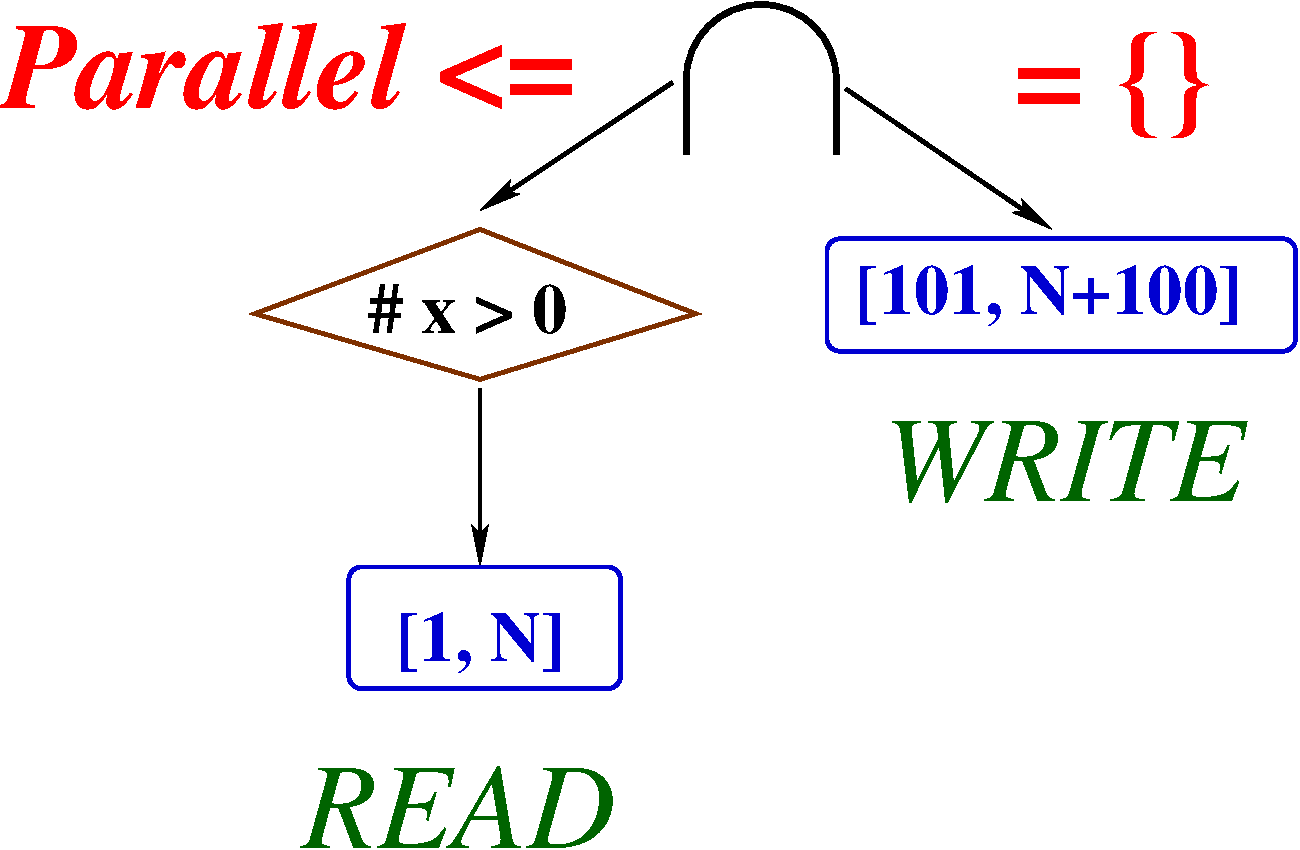
\includegraphics[height=13ex]{Figures/SimpleInd}
\end{center}
\end{columns}
\end{block}
 


%1. Unified Set Reference (USR) [Rus,Rauchwerger,Hoeflinger,2003].\\
%2. Extract a sufficient condition for parallelism, in our case
%{\tt $x\leq 0$~$\vee$~$N \leq 100$} \mymath{\Rightarrow} PARALLEL

Sufficient condition for parallelism: {\tt $x\leq 0$~$\vee$~$N \leq 100$} \mymath{\Rightarrow} PARALLEL.

\end{frame}


\begin{frame}[fragile,t]
  \frametitle{Intuition and Motivation of the Approach}

\begin{block}{Approach Centered on Extracting Arbitrarily Shaped Predicates:} 
\begin{columns}
\column{0.25\textwidth}
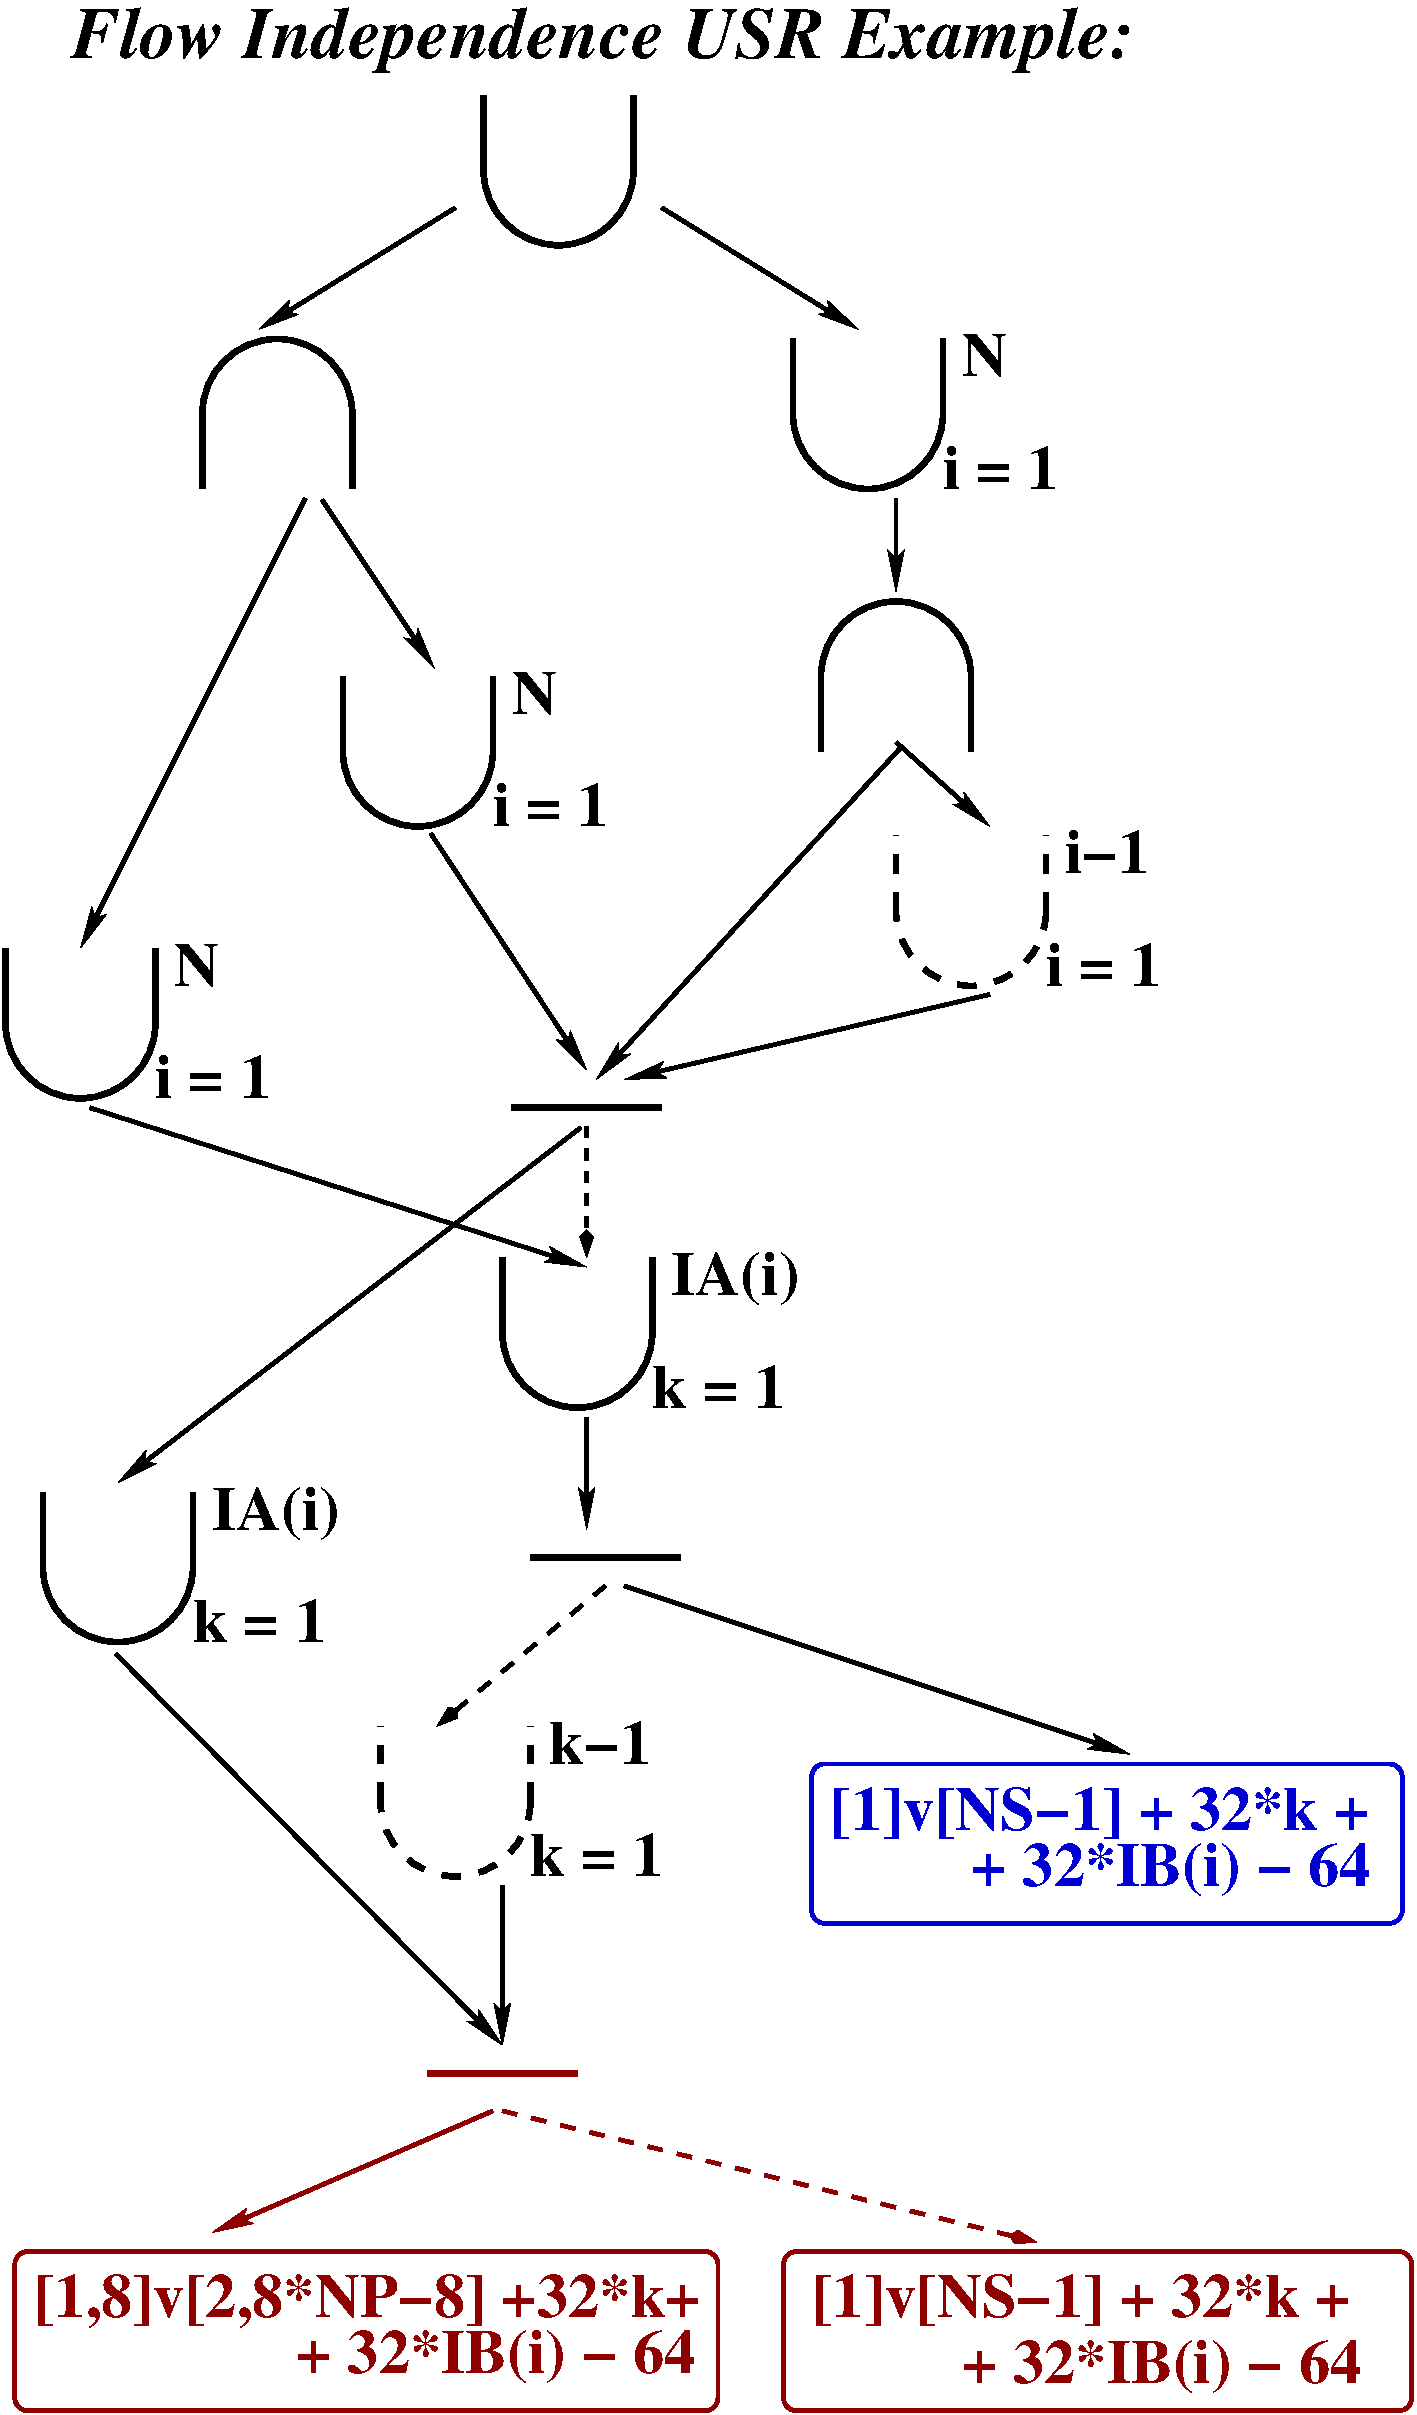
\includegraphics[height=28ex]{Figures/USR_HE_FIND_SOLVH}
\column{0.73\textwidth}\vspace{-1ex}
\begin{itemize}
    \item \emp{\em Parallelism is often dataset sensitive.}\pause\medskip
    \item \emp{{\em Source of inaccuracy:}} summary repres not closed under composition w.r.t. set operations, leads to early conservative approx.\pause \medskip
    \item \emph{{\em Language}} representation for summaries ... precise but \emp{expensive} to compute at runtime \pause \medskip
    \item ``Let's \emph{{\em reason}} about it!'' $S=\emptyset$ $\Leftarrow$ $\emp{A - B} = \emptyset \Leftarrow$ \emph{$8*NP < NS + 6$}!
\end{itemize}
\end{columns}
\end{block}


%{\tiny S.~Rus, L.~Rauchwerger and J.~Hoeflinger, ``Hybrid analysis: static \& dynamic memory reference analysis'', IJPP'03.}\\
{\tiny C.~E.~Oancea and L.~Rauchwerger, ''A Hybrid Approach to Proving Memory Reference Monotonicity'', LCPC'11.}\\
{\tiny C.~E.~Oancea and L.~Rauchwerger, ''Logical Inference Techniques for Loop Parallelization'', PLDI'12.}\\
{\tiny C.~E.~Oancea and L.~Rauchwerger, ''Scalable Conditional Induction Variable (CIV) Analysis'', CGO'15.}

\end{frame}


\begin{frame}[fragile,t]
  \frametitle{Main Steps in Hybrid (static + dynamic) Analysis}
%  \frametitle{Paper's Approach Overview}

Extraction of arbitrary predicates of ``quasi-optimal'' complexity:
%that prove loop independence.
\begin{itemize}

    \item \emph{{\em Language}} to represent summaries: use $-, \cap, \cup_{i=1}^N$, gate, callsite
            nodes when operations fall outside the array-abstraction domain.\smallskip
    
    \item \emph{{\em Translate}} to a language of predicates ($\wedge_{i=1}^{N}, \vee$) \\
            $\mbox{ }\mbox{ }\mbox{ }\mbox{ }\mbox{ }\mbox{ }\mbox{ }$
                \emph{$\mathcal{F} : Summary \rightarrow Predicate$  $\mbox{ }\mbox{ }\mbox{ }$ 
                $S = \emptyset \mbox{ }\Leftarrow\mbox{ }\mathcal{F}(S)$}. \smallskip

    \item The result is factorized into a cascade of predicates, which are \\
            tested at runtime in the order of their estimated complexity. \smallskip

\end{itemize}


{\tiny S.~Rus, L.~Rauchwerger and J.~Hoeflinger, ``Hybrid analysis: static \& dynamic memory reference analysis'', IJPP'03.}\\\smallskip
{\tiny C.~E.~Oancea and L.~Rauchwerger, ''A Hybrid Approach to Proving Memory Reference Monotonicity'', LCPC'11.}\\\smallskip
{\tiny C.~E.~Oancea and L.~Rauchwerger, ''Logical Inference Techniques for Loop Parallelization'', PLDI'12.}\\\smallskip
{\tiny C.~E.~Oancea and L.~Rauchwerger, ''Scalable Conditional Induction Variable (CIV) Analysis'', CGO'15.}\\\smallskip

\end{frame}


\begin{frame}[fragile,t]
  \frametitle{Building RO, RW, WF Summaries Interprocedurally}

Summaries ({\sc ro}, {\sc rw}, {\sc wf}) are
\begin{itemize}
    \item constructed via a bottom-up parse of the \textsc{AbSyn},
    \item structural data-flow equations dictate how to compose consecutive regions,
            aggregate/translate across loops/callsites, ...
\end{itemize}

\pause

\begin{block}{Simplified {\tt solvh\_do20} from {\tt dyfesm}} \vspace{-1ex}
\begin{columns} 
\column{0.45\textwidth}
\begin{colorcode}[fontsize=\scriptsize]
\emp{DO i = 1, N}
    CALL geteu (XE(IA(i)), NP, SYM)
    CALL matmul(XE(IA(i)), NS)
\emp{ENDDO}

SUBROUTINE matmul(XE, NS)
  INTEGER NS, XE(*)
  DO j = 1, NS
    ...   = XE(j) ...
    XE(j) = ...
  ENDDO 
END
\end{colorcode}
\column{0.45\textwidth} 
\begin{colorcode}[fontsize=\scriptsize]
SUBROUTINE geteu(XE, NP, SYM)
  INTEGER NP, SYM, XE(16, *)
  
  IF (SYM .NE. 1) THEN
    DO i = 1, NP
      DO j = 1, 16
        XE(j, i) = ...
      ENDDO 
    ENDDO
  ENDIF
END
\end{colorcode}
\end{columns}
\end{block}

\end{frame}


%%%%%%%%%%%%%%%%%%%%%%%%%%%%%%
%%%%% SUBROUTINE getue
%%%%%%%%%%%%%%%%%%%%%%%%%%%%%%

\begin{frame}[fragile,t]
  \frametitle{Summarizing Subroutine {\tt geteu}}

\begin{block}{WF summary for {\tt geteu}; RO$_{geteu}$ $=$ RW$_{geteu}$ $= \emptyset$ } \vspace{-1ex}
\begin{columns} 
\column{0.45\textwidth} 
\begin{colorcode}[fontsize=\scriptsize]
\mymath{S\myindx{geteu}}  SUBROUTINE geteu(XE, NP, SYM)
         INTEGER NP, SYM, XE(16, *)  
\mymath{S\myindx{IF}}       \emph{IF (SYM .NE. 1) THEN}
\mymath{S\myindx{Li}}         \emp{DO i = 1, NP}
\mymath{S\myindx{Lj}}           \emp{DO j = 1, 16}
\mymath{S\myindx{WF}}             \alert{XE(j, i)} = ...
             \emp{ENDDO} 
           \emp{ENDDO}
         \emph{ENDIF}
       END
\end{colorcode}
\column{0.45\textwidth}
\begin{colorcode}[fontsize=\scriptsize]








\alert{\mymath{WF\myindu{XE}\myindx{S\myindx{WF}} = \{16*i+j-1\}}}
\end{colorcode}
\end{columns}
\end{block}


\begin{itemize}
    \item Loop Aggregation uses (intuitively) interval arithmetic: \smallskip
    \item Loop $j$: $\{16*i + j - 1 \mbox{ }\mbox{ }|\mbox{ } j \in \{1..\mbox{ }16\}\} \rightarrow \emp{16*i + [0,15]}$ \smallskip
    \item Loop $i$: $\{16*i + [0,15] \mbox{ }|\mbox{ } i \in \{1..NP\}\} \rightarrow \emp{[0, 16*NP-1]}$  \smallskip
    \item Branches introduce predicated nodes, e.g., \emph{$WF^{XE}_{S_{if}} = WF^{XE}_{S_{geteu}}$} 
\end{itemize}
\end{frame}

%%%%%%%%%%%%%%%%%%%%%%%%%%%%%%%%%%%%%%%%%%%%%%%%%%%%

\begin{frame}[fragile,t]
  \frametitle{Summarizing Subroutine {\tt geteu}}

\begin{block}{WF summary for {\tt geteu}; RO$_{geteu}$ $=$ RW$_{geteu}$ $= \emptyset$ } \vspace{-1ex}
\begin{columns} 
\column{0.45\textwidth} 
\begin{colorcode}[fontsize=\scriptsize]
\mymath{S\myindx{geteu}}  SUBROUTINE geteu(XE, NP, SYM)
         INTEGER NP, SYM, XE(16, *)  
\mymath{S\myindx{IF}}       \emph{IF (SYM .NE. 1) THEN}
\mymath{S\myindx{Li}}         \emp{DO i = 1, NP}
\mymath{S\myindx{Lj}}           \emp{DO j = 1, 16}
\mymath{S\myindx{WF}}             \alert{XE(j, i)} = ...
             \emp{ENDDO} 
           \emp{ENDDO}
         \emph{ENDIF}
       END
\end{colorcode}
\column{0.45\textwidth}
\begin{colorcode}[fontsize=\scriptsize]






\emp{\mymath{WF\myindu{XE}\myindx{S\myindx{Lj}} = 16*i + [0,15]}}

\alert{\mymath{WF\myindu{XE}\myindx{S\myindx{WF}} = \{16*i+j-1\}}}
\end{colorcode}
\end{columns}
\end{block}


\begin{itemize}
    \item Loop Aggregation uses (intuitively) interval arithmetic: \smallskip
    \item Loop $i$: $\{16*i + j - 1 \mbox{ }\mbox{ }|\mbox{ } j \in \{1..\mbox{ }16\}\} \rightarrow \emp{16*i + [0,15]}$ \smallskip
    \item Loop $j$: $\{16*i + [0,15] \mbox{ }|\mbox{ } i \in \{1..NP\}\} \rightarrow \emp{[0, 16*NP-1]}$  \smallskip
    \item Branches introduce predicated nodes, e.g., \emph{$WF^{XE}_{S_{if}} = WF^{XE}_{S_{geteu}}$} 
\end{itemize}
\end{frame}


%%%%%%%%%%%%%%%%%%%%%%%%%%%%%%%%%%%%%%%%%%%%%%%%%%%%

\begin{frame}[fragile,t]
  \frametitle{Summarizing Subroutine {\tt geteu}}

\begin{block}{WF summary for {\tt geteu}; RO$_{geteu}$ $=$ RW$_{geteu}$ $= \emptyset$ } \vspace{-1ex}
\begin{columns} 
\column{0.45\textwidth} 
\begin{colorcode}[fontsize=\scriptsize]
\mymath{S\myindx{geteu}}  SUBROUTINE geteu(XE, NP, SYM)
         INTEGER NP, SYM, XE(16, *)  
\mymath{S\myindx{IF}}       \emph{IF (SYM .NE. 1) THEN}
\mymath{S\myindx{Li}}         \emp{DO i = 1, NP}
\mymath{S\myindx{Lj}}           \emp{DO j = 1, 16}
\mymath{S\myindx{WF}}             \alert{XE(j, i)} = ...
             \emp{ENDDO} 
           \emp{ENDDO}
         \emph{ENDIF}
       END
\end{colorcode}
\column{0.45\textwidth}
\begin{colorcode}[fontsize=\scriptsize]




\emp{\mymath{WF\myindu{XE}\myindx{S\myindx{Li}} = [0,16*NP-1]}}

\emp{\mymath{WF\myindu{XE}\myindx{S\myindx{Lj}} = 16*i + [0,15]}}

\alert{\mymath{WF\myindu{XE}\myindx{S\myindx{WF}} = \{16*i+j-1\}}}
\end{colorcode}
\end{columns}
\end{block}


\begin{itemize}
    \item Loop Aggregation uses (intuitively) interval arithmetic: \smallskip
    \item Loop $i$: $\{16*i + j - 1 \mbox{ }\mbox{ }|\mbox{ } j \in \{1..\mbox{ }16\}\} \rightarrow \emp{16*i + [0,15]}$ \smallskip
    \item Loop $j$: $\{16*i + [0,15] \mbox{ }|\mbox{ } i \in \{1..NP\}\} \rightarrow \emp{[0, 16*NP-1]}$  \smallskip
    \item Branches introduce predicated nodes, e.g., \emph{$WF^{XE}_{S_{if}} = WF^{XE}_{S_{geteu}}$} 
\end{itemize}
\end{frame}


%%%%%%%%%%%%%%%%%%%%%%%%%%%%%%%%%%%%%%%%%%%%%%%%%%%%

\begin{frame}[fragile,t]
  \frametitle{Summarizing Subroutine {\tt geteu}}

\begin{block}{WF summary for {\tt geteu}; RO$_{geteu}$ $=$ RW$_{geteu}$ $= \emptyset$ } \vspace{-1ex}
\begin{columns} 
\column{0.45\textwidth} 
\begin{colorcode}[fontsize=\scriptsize]
\mymath{S\myindx{geteu}}  SUBROUTINE geteu(XE, NP, SYM)
         INTEGER NP, SYM, XE(16, *)  
\mymath{S\myindx{IF}}       \emph{IF (SYM .NE. 1) THEN}
\mymath{S\myindx{Li}}         \emp{DO i = 1, NP}
\mymath{S\myindx{Lj}}           \emp{DO j = 1, 16}
\mymath{S\myindx{WF}}             \alert{XE(j, i)} = ...
             \emp{ENDDO} 
           \emp{ENDDO}
         \emph{ENDIF}
       END
\end{colorcode}
\column{0.45\textwidth}
\begin{colorcode}[fontsize=\scriptsize]
          \emph{\mymath{(SYM \neq 1)}}
\emph{\mymath{WF\myindu{XE}\myindx{S\myindx{IF}} =}       \mymath{\downarrow}}
          \emph{\mymath{[0,16*NP-1]}}

\emp{\mymath{WF\myindu{XE}\myindx{S\myindx{Li}} = [0,16*NP-1]}}

\emp{\mymath{WF\myindu{XE}\myindx{S\myindx{Lj}} = 16*i + [0,15]}}

\alert{\mymath{WF\myindu{XE}\myindx{S\myindx{WF}} = \{16*i+j-1\}}}
\end{colorcode}
\end{columns}
\end{block}


\begin{itemize}
    \item Loop Aggregation uses (intuitively) interval arithmetic: \smallskip
    \item Loop $i$: $\{16*i + j - 1 \mbox{ }\mbox{ }|\mbox{ } j \in \{1..\mbox{ }16\}\} \rightarrow \emp{16*i + [0,15]}$ \smallskip
    \item Loop $j$: $\{16*i + [0,15] \mbox{ }|\mbox{ } i \in \{1..NP\}\} \rightarrow \emp{[0, 16*NP-1]}$  \smallskip
    \item Branches introduce predicated nodes, e.g., \emph{$WF^{XE}_{S_{if}} = WF^{XE}_{S_{geteu}}$} 
\end{itemize}
\end{frame}


%%%%%%%%%%%%%%%%%%%%%%%%%%%%%%
%%%%% SUBROUTINE getue END
%%%%%%%%%%%%%%%%%%%%%%%%%%%%%%


%%%%% SUBROUTINE MATMULT

\begin{frame}[fragile,t]
  \frametitle{Summarizing Subroutine {\tt matmult}}

\begin{block}{RW summary for {\tt matmul}; RO$_{matmul}$ $=$ WF$_{matmul}$ $= \emptyset$ } \vspace{-1ex}
\begin{columns} 
\column{0.48\textwidth} 
\begin{colorcode}[fontsize=\scriptsize]
\mymath{S\myindx{matmul}}  SUBROUTINE matmul(XE, NS)
          INTEGER NS, XE(*)
\mymath{S\myindx{loop}}       \emph{DO j = 1, NS}
\mymath{S\myindx{RO}}          \alert{...   \hspace{0.5ex}= XE(j) ...}
\mymath{S\myindx{WF}}          \alert{XE(j) = ...}
          \emph{ENDDO}
        END
\end{colorcode}
\column{0.48\textwidth}
\begin{colorcode}[fontsize=\scriptsize]




\alert{\mymath{RO\myindu{XE}\myindx{S\myindx{RO}} = \{j-1\}}}
\alert{\mymath{WF\myindu{XE}\myindx{S\myindx{WF}} = \{j-1\}}}
\end{colorcode}
\end{columns}
\end{block}

\bigskip

\begin{itemize}
    \item Composing read-only $RO_{S_1}$ and write-first $WF_{S_2}$ regions:  \smallskip
    \item $RO = RO_{S_1} - WF_{S_2}$, $WF = WF_{S_2} - RO_{S_1}$, $RW = RO_{S_1} \cap WF_{S_2}$  \smallskip
    \item In our case $RO = \emptyset$, $WF = \emptyset$, \emp{$RW = \{j-1\}$}  \smallskip
    \item Over loop {\tt DO j}:  $RO_{loop} = \emptyset$, $WF_{loop} = \emptyset$, \emph{$RW_{loop} = [0, NS-1]$}  \smallskip
\end{itemize}
\end{frame}

%%%%%%%%%%%%%%%%%%%%%%%%%%%%%%%%%%%%%%%%%%%%%%%%%%%%

%%%%%%%%%%%%%%%%%%%%%%%%%%%%%%%%%%%%%%%%%%%%%%%%%%%%

\begin{frame}[fragile,t]
  \frametitle{Summarizing Subroutine {\tt matmult}}

\begin{block}{RW summary for {\tt matmul}; RO$_{matmul}$ $=$ WF$_{matmul}$ $= \emptyset$ } \vspace{-1ex}
\begin{columns} 
\column{0.48\textwidth} 
\begin{colorcode}[fontsize=\scriptsize]
\mymath{S\myindx{matmul}}  SUBROUTINE matmul(XE, NS)
          INTEGER NS, XE(*)
\mymath{S\myindx{loop}}       \emph{DO j = 1, NS}
\mymath{S\myindx{RO}}          \alert{...   \hspace{0.5ex}= XE(j) ...}
\mymath{S\myindx{WF}}          \alert{XE(j) = ...}
          \emph{ENDDO}
        END
\end{colorcode}
\column{0.48\textwidth}
\begin{colorcode}[fontsize=\scriptsize]


\emp{\mymath{S\myindx{RO} \diamond S\myindx{WF} = \{\emptyset, \emptyset, RW=\{j-1\}\}}}

\alert{\mymath{RO\myindu{XE}\myindx{S\myindx{RO}} = \{j-1\}}}
\alert{\mymath{WF\myindu{XE}\myindx{S\myindx{WF}} = \{j-1\}}}
\end{colorcode}
\end{columns}
\end{block}

\bigskip

\begin{itemize}
    \item Composing read-only $RO_{S_1}$ and write-first $WF_{S_2}$ regions:  \smallskip
    \item $RO = RO_{S_1} - WF_{S_2}$, $WF = WF_{S_2} - RO_{S_1}$, $RW = RO_{S_1} \cap WF_{S_2}$  \smallskip
    \item In our case $RO = \emptyset$, $WF = \emptyset$, \emp{$RW = \{j-1\}$}  \smallskip
    \item Over loop {\tt DO j}:  $RO_{loop} = \emptyset$, $WF_{loop} = \emptyset$, \emph{$RW_{loop} = [0, NS-1]$}  \smallskip
\end{itemize}
\end{frame}


\begin{frame}[fragile,t]
  \frametitle{Summarizing Subroutine {\tt matmult}}

\begin{block}{RW summary for {\tt matmul}; RO$_{matmul}$ $=$ WF$_{matmul}$ $= \emptyset$ } \vspace{-1ex}
\begin{columns} 
\column{0.48\textwidth} 
\begin{colorcode}[fontsize=\scriptsize]
\mymath{S\myindx{matmul}}  SUBROUTINE matmul(XE, NS)
          INTEGER NS, XE(*)
\mymath{S\myindx{loop}}       \emph{DO j = 1, NS}
\mymath{S\myindx{RO}}          \alert{...   \hspace{0.5ex}= XE(j) ...}
\mymath{S\myindx{WF}}          \alert{XE(j) = ...}
          \emph{ENDDO}
        END
\end{colorcode}
\column{0.48\textwidth}
\begin{colorcode}[fontsize=\scriptsize]
\emph{\mymath{RW\myindu{XE}\myindx{S\myindx{loop}} = [0,NS-1]}}

\emp{\mymath{S\myindx{RO} \diamond S\myindx{WF} = \{\emptyset, \emptyset, RW=\{j-1\}\}}}

\alert{\mymath{RO\myindu{XE}\myindx{S\myindx{RO}} = \{j-1\}}}
\alert{\mymath{WF\myindu{XE}\myindx{S\myindx{WF}} = \{j-1\}}}
\end{colorcode}
\end{columns}
\end{block}

\bigskip

\begin{itemize}
    \item Composing read-only $RO_{S_1}$ and write-first $WF_{S_2}$ regions:  \smallskip
    \item $RO = RO_{S_1} - WF_{S_2}$, $WF = WF_{S_2} - RO_{S_1}$, $RW = RO_{S_1} \cap WF_{S_2}$  \smallskip
    \item In our case $RO = \emptyset$, $WF = \emptyset$, \emp{$RW = \{j-1\}$}  \smallskip
    \item Over loop {\tt DO j}:  $RO_{loop} = \emptyset$, $WF_{loop} = \emptyset$, \emph{$RW_{loop} = [0, NS-1]$}  \smallskip
\end{itemize}
\end{frame}



%%%%% SUBROUTINE MATMULT

\begin{frame}[fragile,t]
  \frametitle{Summarizing Accesses for the Target Loop}

\begin{block}{RW summary for loop {\tt DO i}: RW$^i$ = ? } \vspace{-1ex}
\begin{columns} 
\column{0.48\textwidth} 
\begin{colorcode}[fontsize=\scriptsize]
        INTEGER NS, NP, IA(*), XE(*)
\mymath{S\myindx{loop}}    \emph{DO i = 1, N}
\mymath{S\myindx{WF}}      CALL geteu (XE(IA(i)),NP,SYM)
\mymath{S\myindx{RW}}      CALL matmul(XE(IA(i)),NS)
        \emph{ENDDO}

\emp{\mymath{S\myindx{WF} \diamond S\myindx{RW} = \{\emptyset, WF\myindu{i}=WF\myindx{geteu}, RW\myindu{i}\}}}
\end{colorcode}
\column{0.48\textwidth}
\begin{center}
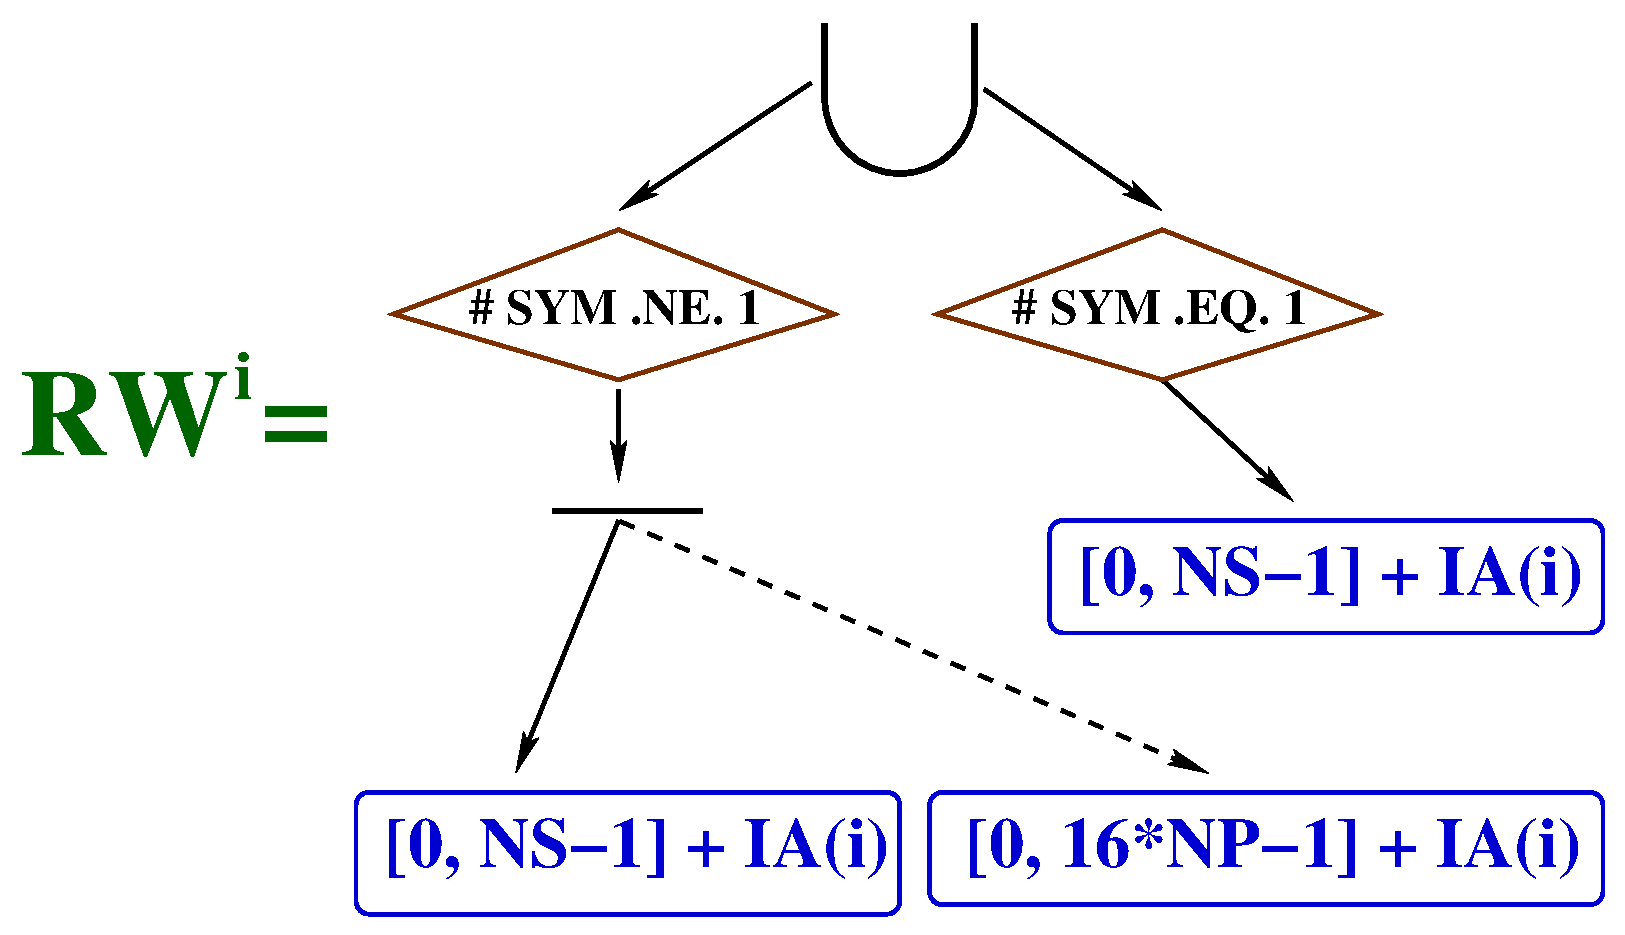
\includegraphics[height=15ex]{Figures/RW_IND_XE}
\end{center}
\end{columns}
\end{block}

\bigskip

\begin{itemize}
    \item Composing write-first $WF^i_{S_1}$ and read-write $RW^i_{S_2}$ regions:  \smallskip
    \item $RO^i = \emptyset$, $WF^i = WF^i_{S_1}$, $RW^i = RW^i_{S_2} - WF^i_{S_1}$  \smallskip
    \item In our case $RO^i = \emptyset$, $WF = WF^i_{geteu}$ not shown, \emph{$RW^{i}$ as above}
\end{itemize}
\end{frame}


%%%%%% Flow-Anti Independence Summary-Based Equation

\begin{frame}[fragile,t]
  \frametitle{Summary-Based Independence Equations}
\bigskip
Flow and Anti Independence Equation for loop of index \emph{i}:
\begin{equation} \label{FIEq} 
\begin{array}{l r}
S_{find} = \{(\cup_{i=1}^{N} WF_i) \mbox{ }\cap\mbox{ } (\cup_{i=1}^{N} RO_i)\} \mbox{ }\cup & \vspace{1ex} \\ \mbox{ }\mbox{ }\mbox{ }\mbox{ }\mbox{ }\mbox{ }\mbox{ }\mbox{ }\mbox{ }\mbox{ }
\{(\cup_{i=1}^{N} WF_i) \mbox{ }\cap\mbox{ } (\cup_{i=1}^{N} RW_i)\} \mbox{ }\cup & \vspace{1ex} \\ \mbox{ }\mbox{ }\mbox{ }\mbox{ }\mbox{ }\mbox{ }\mbox{ }\mbox{ }\mbox{ }\mbox{ }
\{(\cup_{i=1}^{N}RO_i) \mbox{ }\cap\mbox{ } (\cup_{i=1}^{N}RW_i)\} \mbox{ }\cup  & \vspace{1ex} \\ \mbox{ }\mbox{ }\mbox{ }\mbox{ }\mbox{ }\mbox{ }\mbox{ }\mbox{ }\mbox{ }\mbox{ }
\{ \cup_{i=1}^{N}(RW_i \mbox{ }\cap\mbox{ } (\cup_{k=1}^{i-1}RW_k))\} \mbox{ }\mbox{ }\mbox{ } = \emptyset
\end{array}
\end{equation}

\bigskip

\pause

Output Independence Equation for loop of index \emph{i}:
\begin{equation} \label{OIEq} 
\begin{array}{l r}
S_{oind} = \{ \cup_{i=1}^{N}(WF_i \mbox{ }\cap\mbox{ } (\cup_{k=1}^{i-1}WF_k))\} \mbox{ }\mbox{ }\mbox{ } = \emptyset
\end{array}
\end{equation}

\bigskip

\pause

Computing $S_{find}$ and $S_{oind}$ solves a more difficult problem than we need, 
i.e., computes the indexes involved in cross-iteration deps. \bigskip

\emp{{\em Loop Independence: when are $S_{find}$ and $S_{oind}$ are empty?}}

\end{frame}


%%%% Summary to Predicate Translation

\begin{frame}[fragile,t]
  \frametitle{Predicate Extraction via Logical Inference Rules}

Translation Scheme $\mathcal{F}$ from summary to predicate language: \smallskip \\ 
$\mbox{ }\mbox{ }\mbox{ }\mbox{ }\mbox{ }$ $\mathcal{F} : Summary \rightarrow Predicates$ 
$\mbox{ }\mbox{ }\mbox{ }$  \emp{$S \mbox{ }=\mbox{ } \emptyset \mbox{ }\mbox{ }\mbox{ }\Leftarrow \mbox{ }\mathcal{F}(S)$} \smallskip \\

Predicates constructed via a top-down pass of the indep. summary. \smallskip 

\pause

\begin{block}{ Translating the Flow-Independence Summary for {\tt XE} in {\tt solh\_do20} } \vspace{-1ex}
\begin{columns} 
\column{0.60\textwidth} 
\begin{itemize}
    \item Assume $S_{ind}=\emptyset$ indep. equation: \smallskip \\
$\cup_{i=1}^{N}(RW_i \mbox{ }\cap\mbox{ } (\cup_{k=1}^{i-1}RW_k))=\emptyset$  \bigskip

    \item \emph{Rule: $\cup_{i=1}^{N}S_{i}=\emptyset \mbox{ }\Leftarrow\mbox{ } \wedge^N_{i=1}\mathcal{F}(S_i)$} \pause \bigskip

    \item \emp{$\mbox{ }\mbox{ }\mbox{ }\mbox{ }\mbox{ }\mathcal{F}(\mbox{ }RW_i \mbox{ }\cap\mbox{ } (\cup_{k=1}^{i-1}RW_k)\mbox{ }) = ?$}  \bigskip

    \item \emph{Rule: $S_1 \mbox{ }\cap\mbox{ } S_2 = \emptyset \mbox{ }\Leftarrow\mbox{ }\mathcal{F}(S_1) \vee ... $} \pause \bigskip

    \item \emp{$\mbox{ }\mbox{ }\mbox{ }\mbox{ }\mbox{ }\mathcal{F}(RW_i) = ?$}
\end{itemize}
\column{0.35\textwidth} 
\begin{center} \hspace{-4ex}
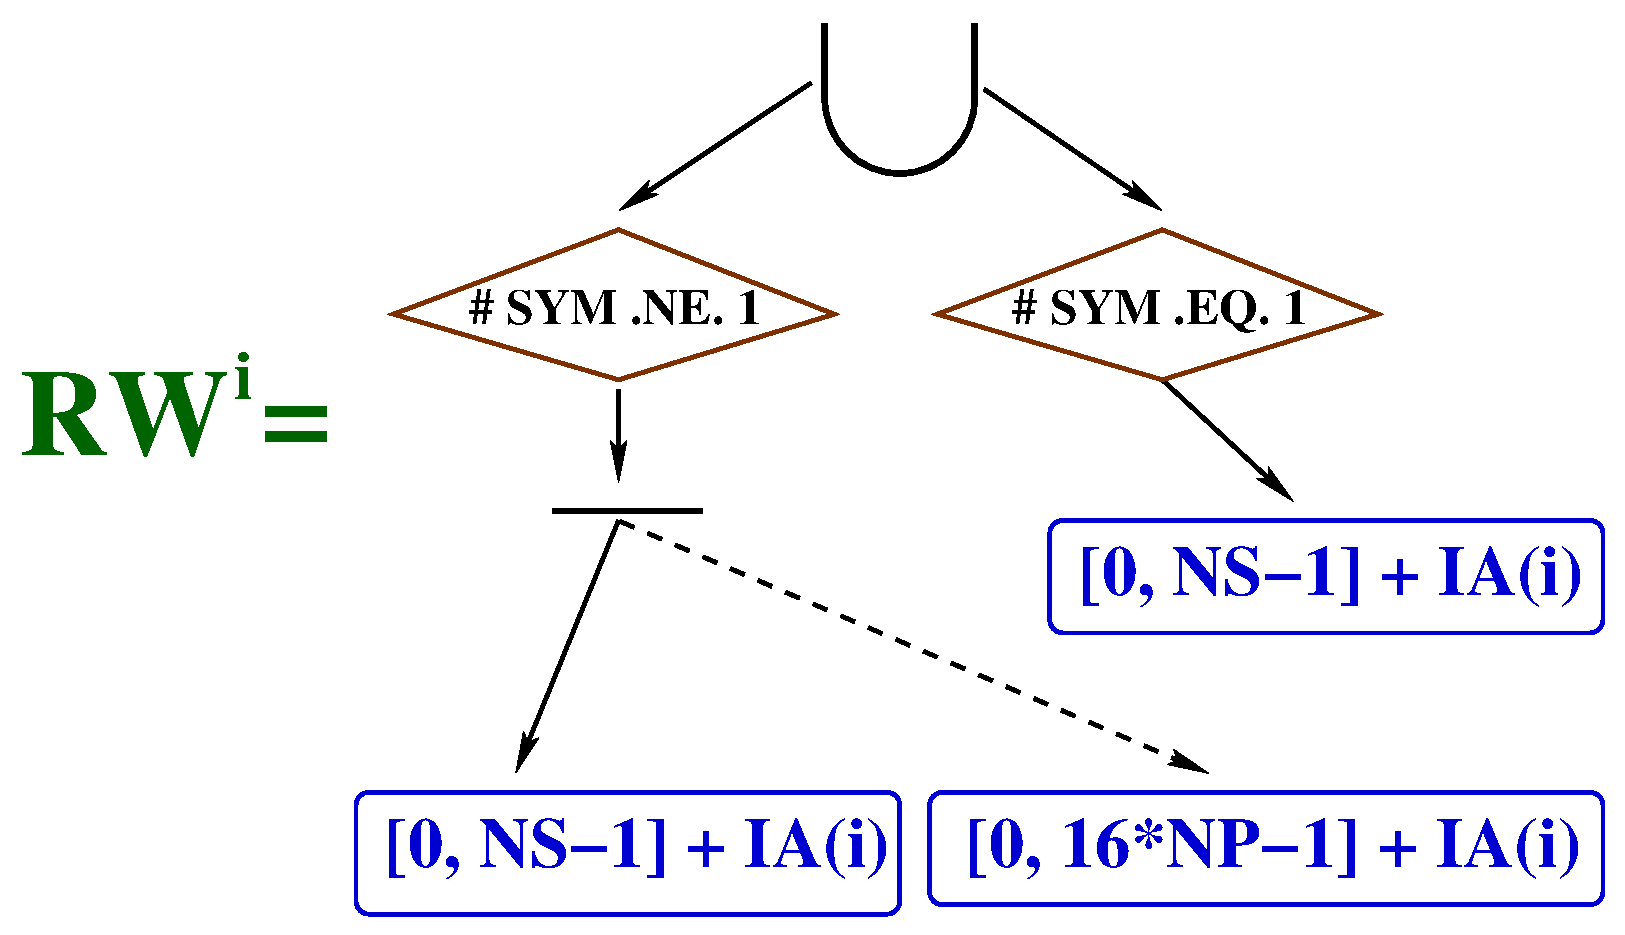
\includegraphics[height=15ex]{Figures/RW_IND_XE}
\end{center}
\end{columns}
\end{block}

\end{frame}

%%%%%%%%%%%%%%%%%%%%%%%%%%%%%

\begin{frame}[fragile,t]
  \frametitle{Summary to Predicate Translation}

\begin{center} \hspace{-9ex}
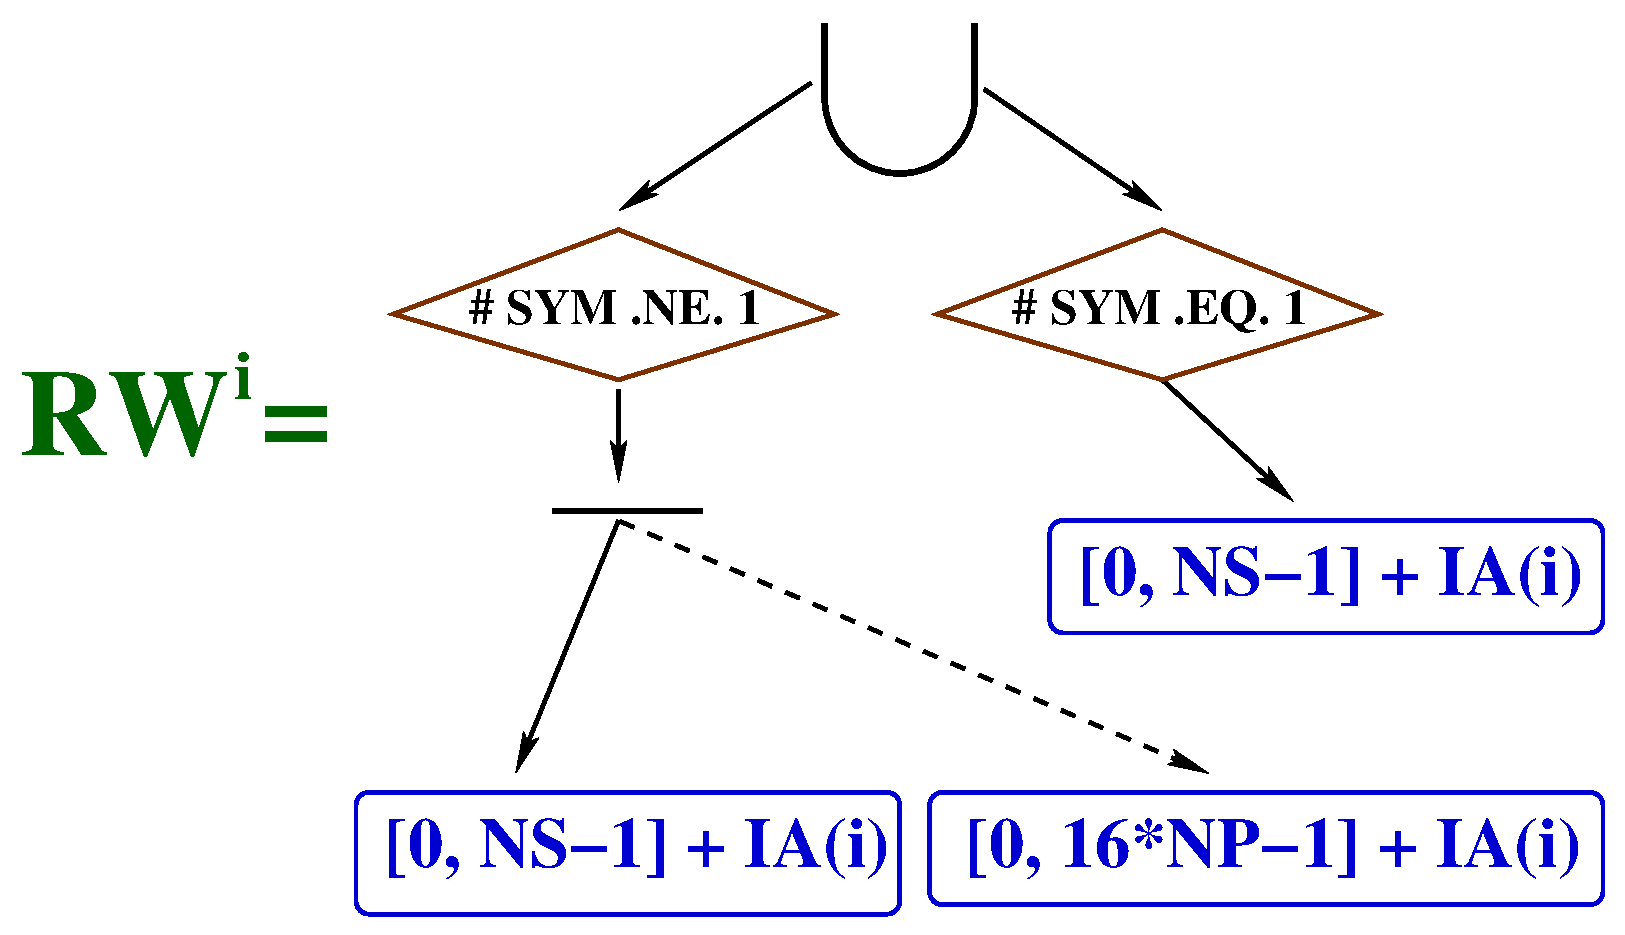
\includegraphics[height=17ex]{Figures/RW_IND_XE}
\end{center}

A sufficient {\tt XE}-independence condition is: \bigskip \\ 
$\mathcal{F}(\cup_{i=1}^{N}(RW_i \mbox{ }\cap\mbox{ } (\cup_{k=1}^{i-1}RW_k))) =$ 
%$\mbox{ }\mbox{ }\mbox{ }\mbox{ }\mbox{ }$
\emph{$\wedge_{i=1}^N(\mbox{ }{\tt SYM}\neq 1\mbox{ }\wedge {\tt NS}\leq 16*{\tt NP}\mbox{ })$} 

\bigskip
\bigskip

We have shown just the trivial logical inference rules.\\
For example, more complex ones exploit indirect-array monotonicity. 

%\begin{columns}
%\column{0.60\textwidth}
%$\mbox{ }$ \\
%A sufficient {\tt XE}-independence condition is: \smallskip \\ 
%$\mathcal{F}(\cup_{i=1}^{N}(RW_i \mbox{ }\cap\mbox{ } (\cup_{k=1}^{i-1}RW_k))) =$ \bigskip \\
%$\mbox{ }\mbox{ }\mbox{ }\mbox{ }\mbox{ }$
%\emph{$\wedge_{i=1}^N(\mbox{ }{\tt SYM}\neq 1\mbox{ }\wedge {\tt NS}\leq 16*{\tt NP}\mbox{ })$} 
%\column{0.35\textwidth} 
%\begin{center} \hspace{-9ex}
%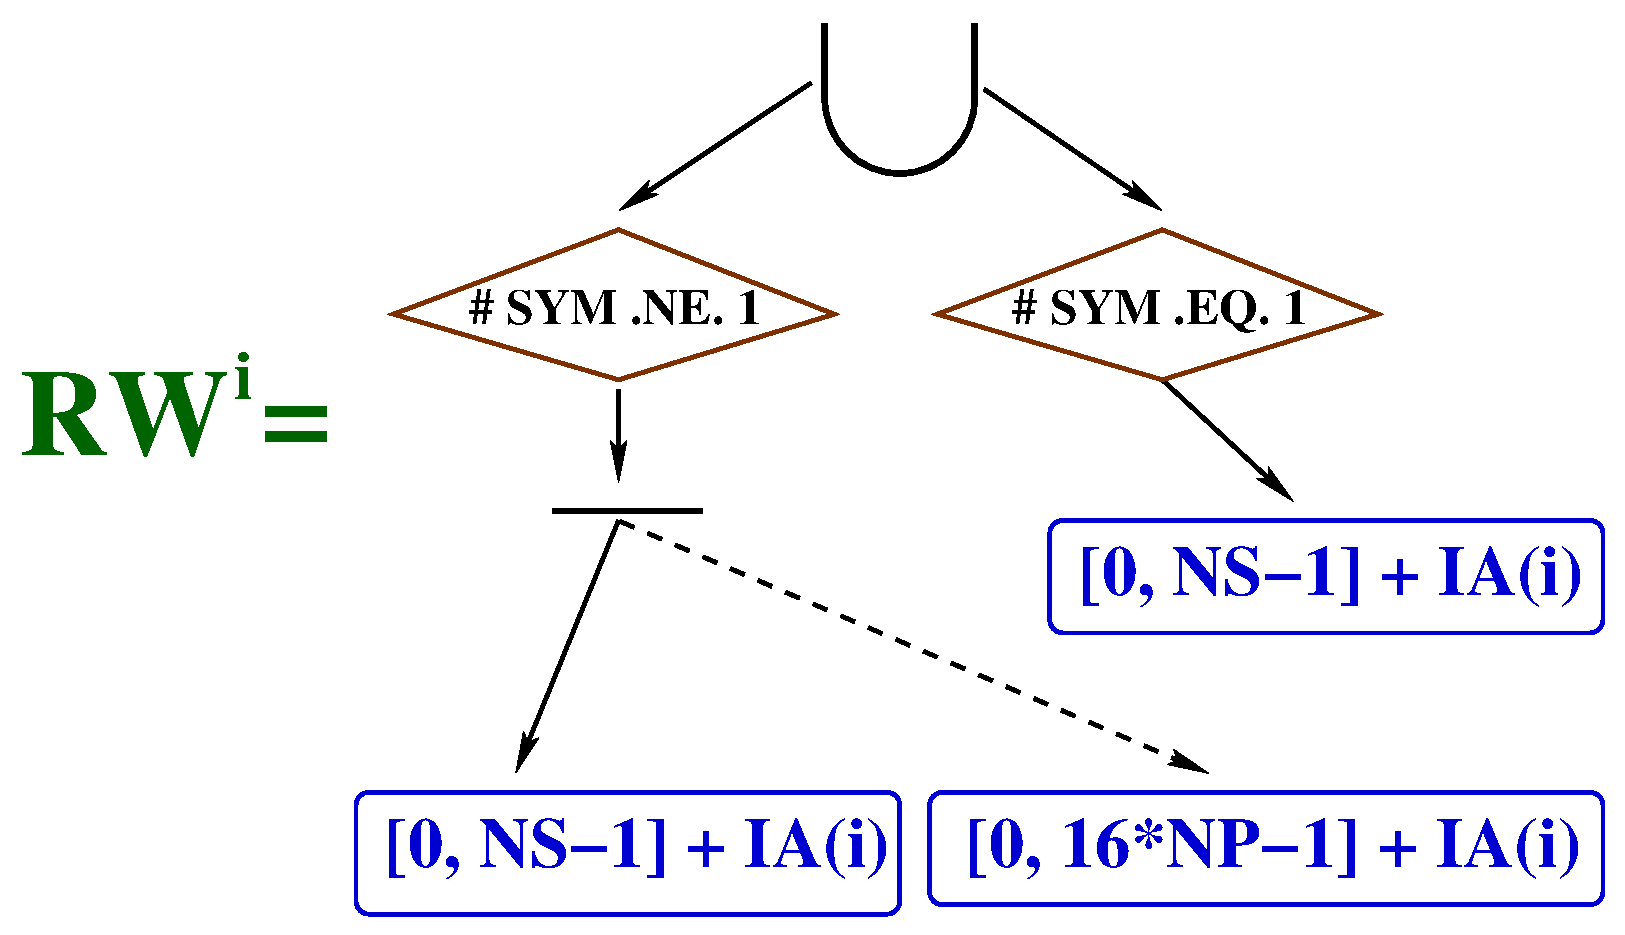
\includegraphics[height=17ex]{Figures/RW_IND_XE}
%\end{center}
%\end{columns}


\end{frame}


\begin{frame}[fragile,t]
  \frametitle{Predicate Simplification/Extraction Techniques}

\bigskip
\emp{{\em Predicate Simplifications:}}
\begin{itemize}
    \item Invariant Hoisting: $\emp{\wedge_{i=1}^{N}}(\vee(\emp{A_1^{inv}, .., A_r^{inv}}, B_1^{var}, .., B_p^{var})) \rightarrow$ \smallskip \\
            $\mbox{ }\mbox{ }\mbox{ }\mbox{ }$ $\emph{(\vee(A_1^{inv}, .., A_r^{inv}))}\mbox{ }\vee\mbox{ } (\wedge_{i=1}^{N}(\vee(B_1^{var}, .., B_p^{var})))$ \pause \smallskip
    \item With our example: \emp{$\wedge_{i=1}^N(\mbox{ }{\tt SYM}\neq 1\mbox{ }\wedge {\tt NS}\leq 16*{\tt NP}\mbox{ })$} $\rightarrow$ \smallskip \\ $\mbox{ }\mbox{ }\mbox{ }\mbox{ }$ \emph{${\tt SYM}\neq 1\mbox{ }\wedge {\tt NS}\leq 16*{\tt NP}$}, which is $O(1)$ runtime.  
\end{itemize}

\bigskip

\pause

\emp{{\em Predicate Extraction:}}
\begin{itemize}
    \item To extract $O(1)$ predicates, apply aggressive-invariant rules : \smallskip \\
            $\emp{\wedge_{i=1}^{N}}(\wedge(\emp{A_1^{inv}}\vee B_1^{var}, .., \emp{A_p^{inv}} \vee B_p^{var}))$  \emph{$\mbox{ }\mbox{ }\mbox{ }\rightarrow\mbox{ }\wedge(A_1^{inv}, .., A_p^{inv})$} \pause \bigskip

    \item To extract $O(N)$ predicates: replace inner-loop nodes with {\tt false} and simplify the result.
\end{itemize}

\end{frame}


\begin{frame}[fragile,t]
  \frametitle{Extracting $O(N)$ Predicates Example}

\bigskip

\begin{columns} 
\column{0.50\textwidth} 
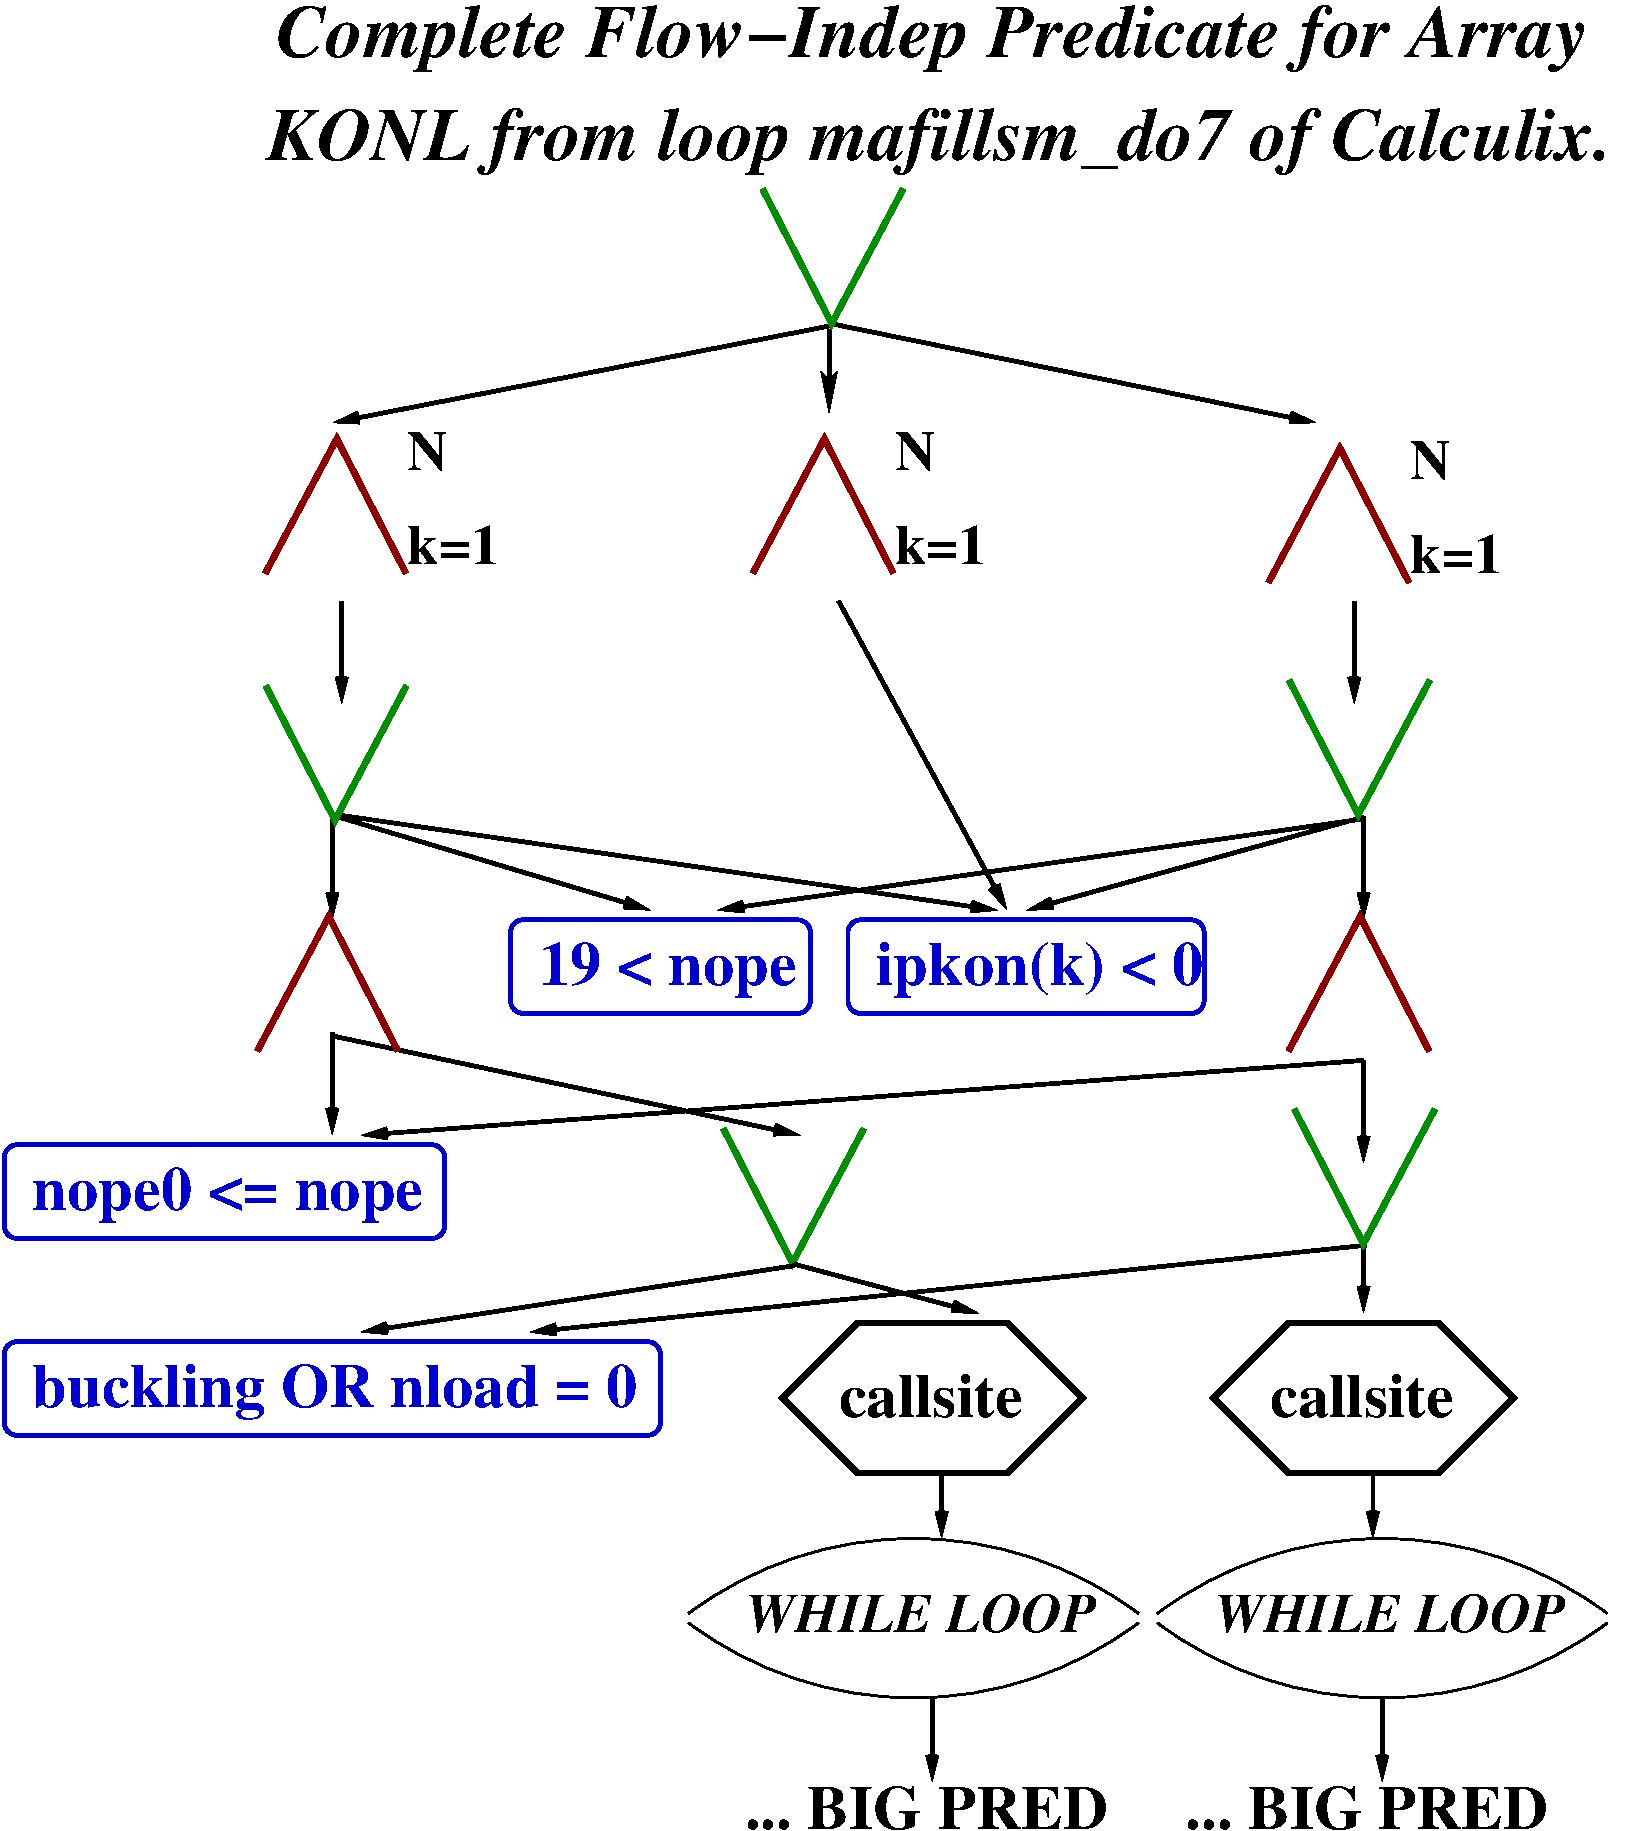
\includegraphics[height=39ex]{Figures/CALCULIX_PDAG1}
\column{0.48\textwidth} 
Approximating the while loops with {\tt false} nodes and simplifying yields $O(N)$ predicate: 

\bigskip

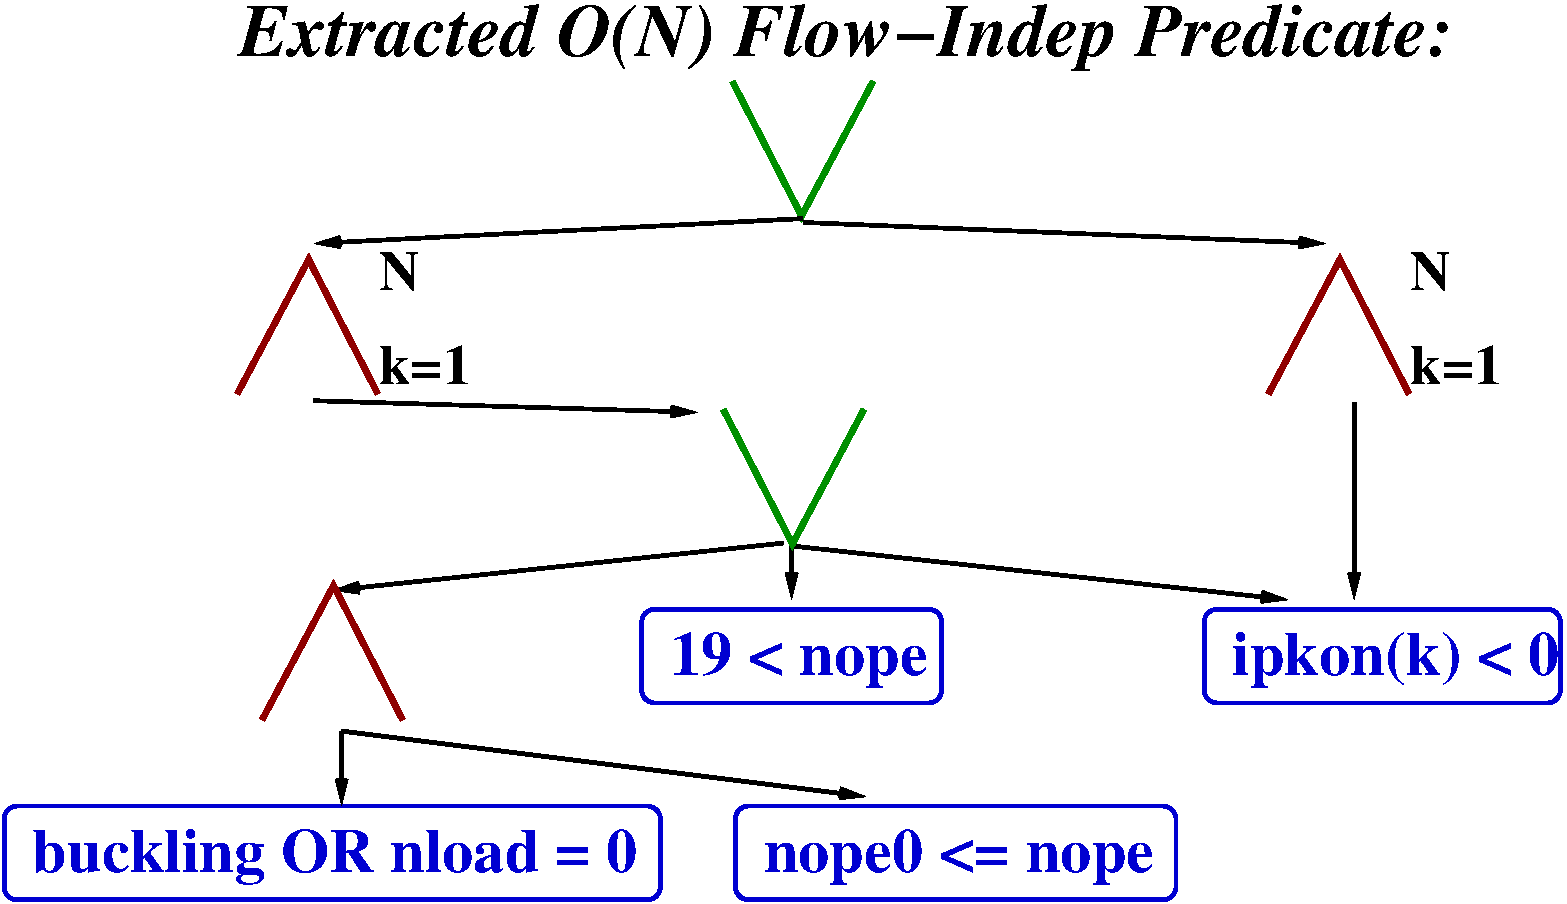
\includegraphics[height=20ex]{Figures/CALCULIX_PDAG2}
\end{columns}


\end{frame}

%%%%%%%%%%%%% Predicate Simplification
% and Factorization
%\begin{frame}[fragile,t]
%  \frametitle{Enabling Transformations for Predicate Extraction}
%
%\emp{{\em Summary Transformations:}}
%
%\begin{itemize}
%    \item ``Strength Reduction:'' union preferred to repeated subtraction,
%    \item Preserving the shape of a Union of Mutually Exclusive Gates.
%\end{itemize}
%
%\bigskip
%
%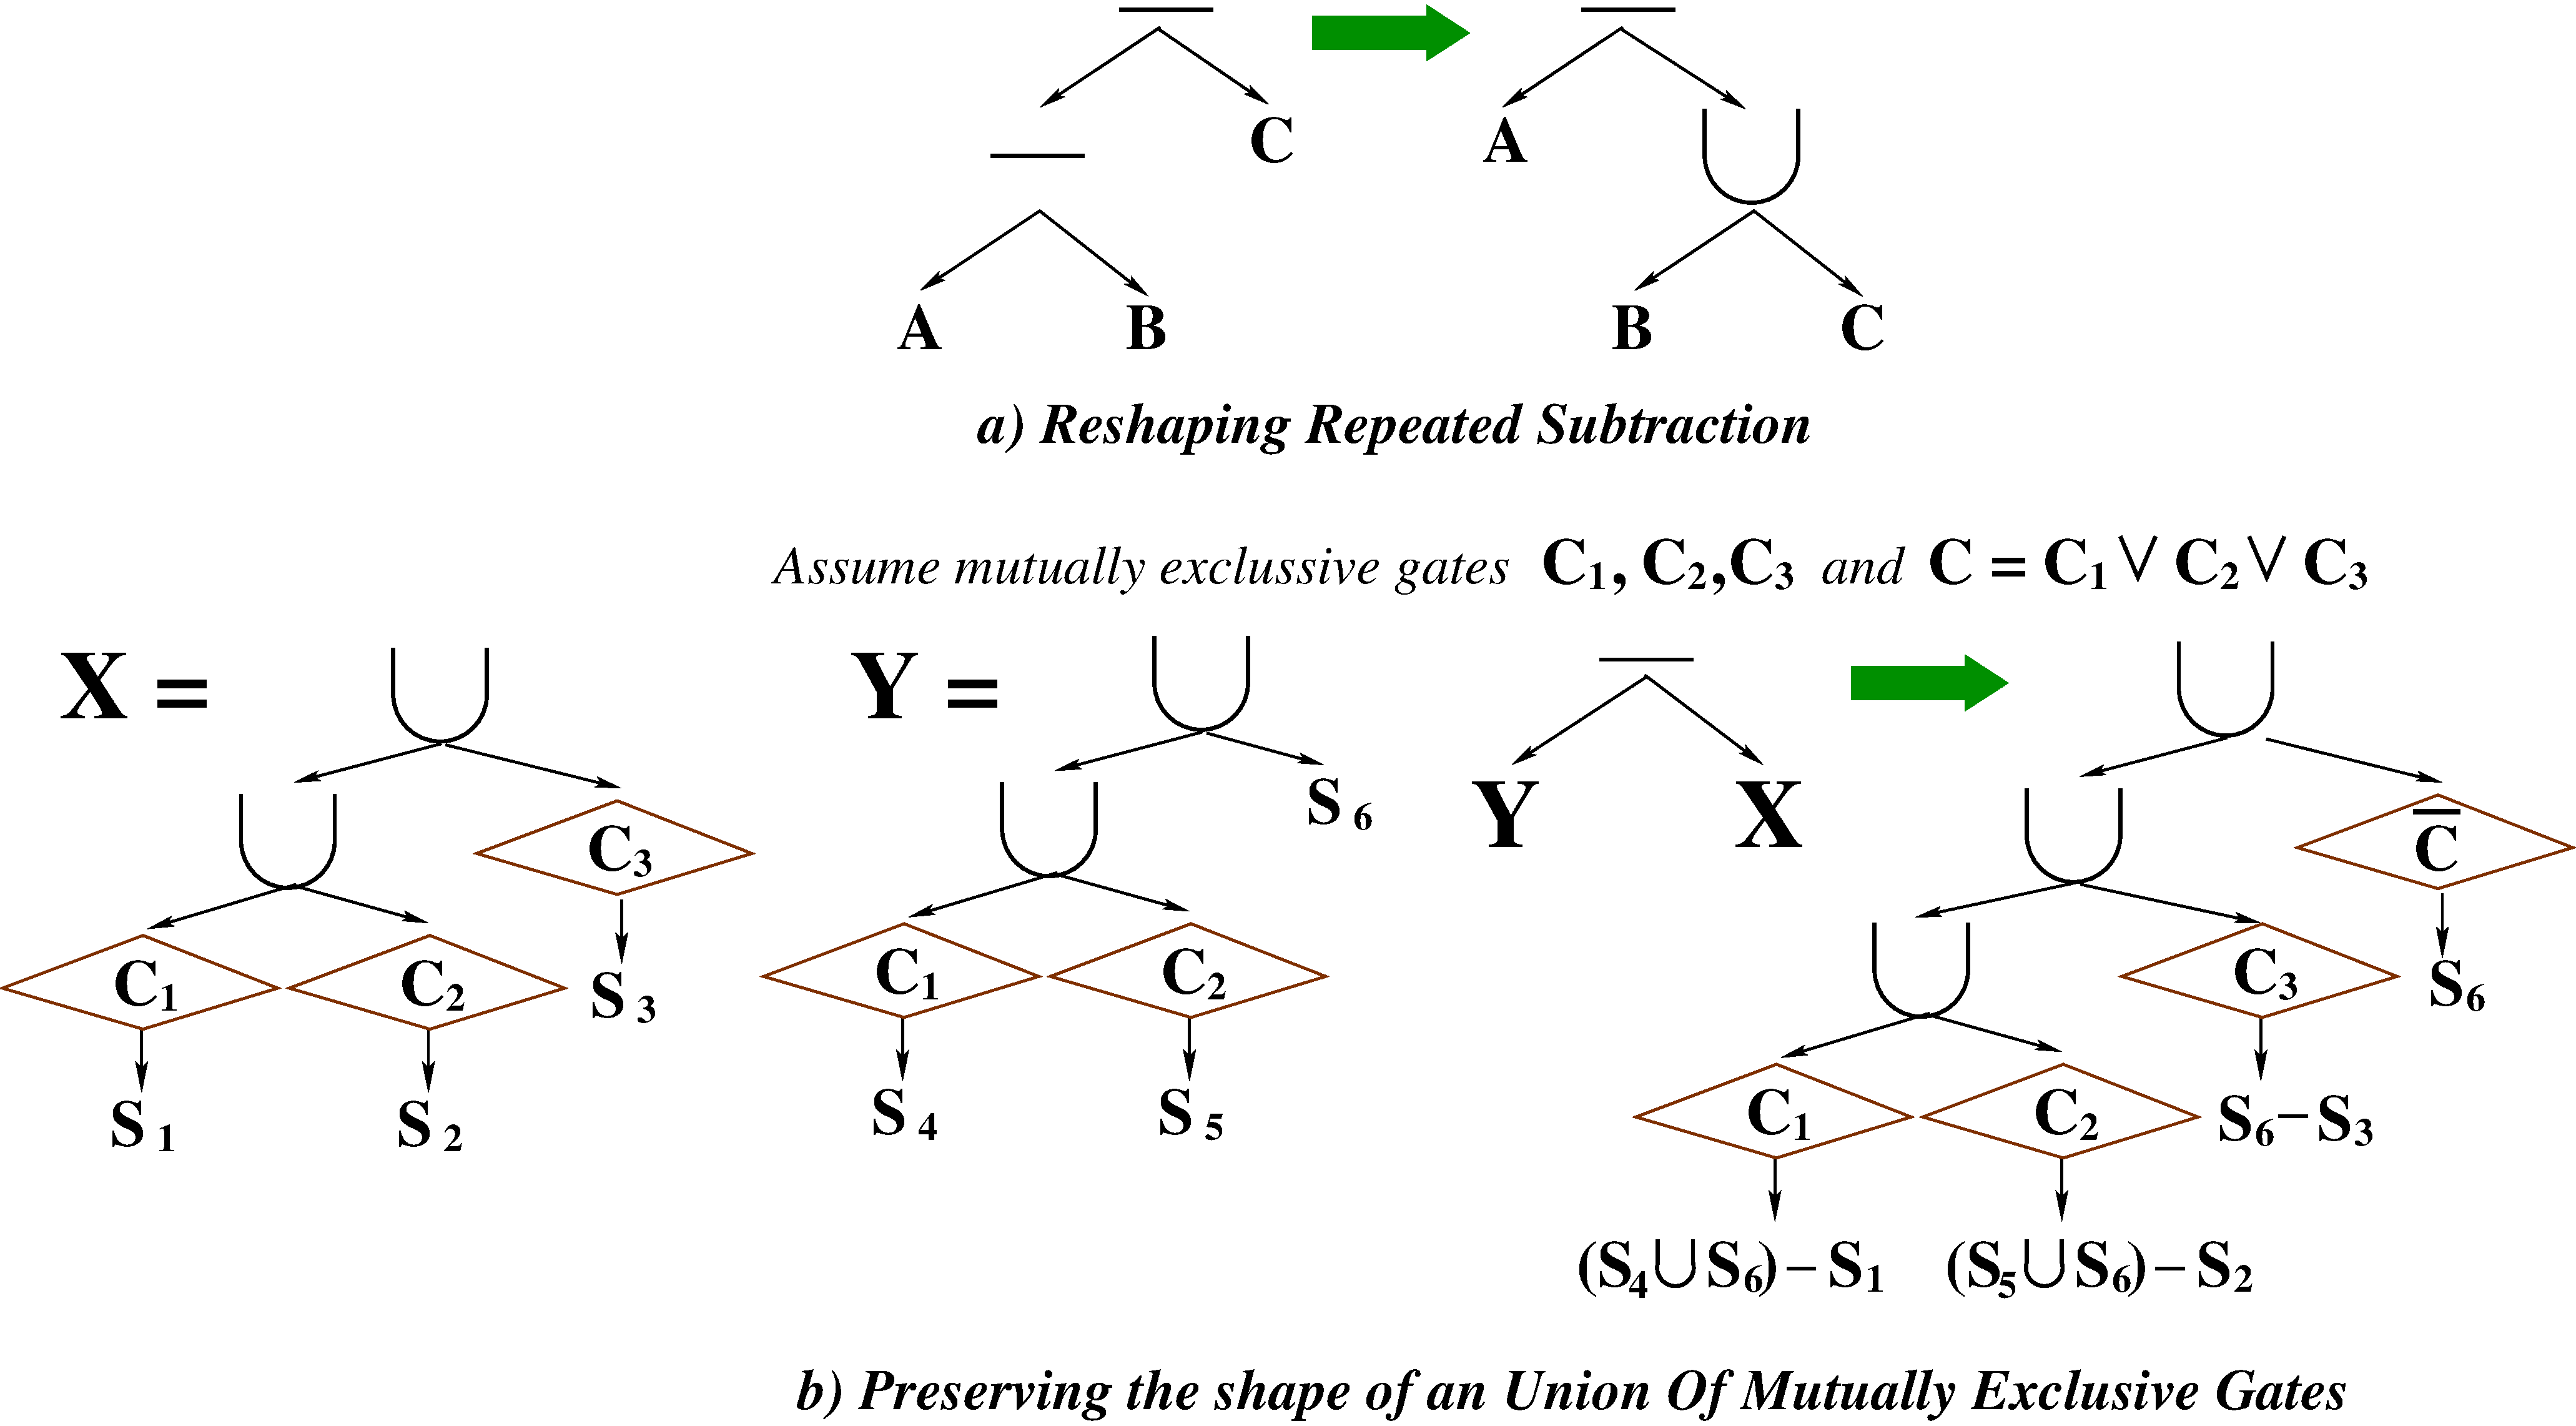
\includegraphics[height=31ex]{Figures/USR_RESHAPE_TARNSF}
%
%\end{frame}


%%% Non-trivial Rules for Deriving Predicates


\begin{frame}[fragile,t]
  \frametitle{Are We Done Already?}

\alert{NO!}
\bigskip

\begin{itemize}
    \item These were the ``simple'' examples ...\\ 
            solved uglier ones still at negligible overhead,\\
            see for example {\tt Figures/IND\_PRED/indequ.pdf}.\bigskip

    \item Code Generation for the predicate nontrivial:
            \begin{itemize}
                \item program slice containing predicate's symbols
                \item insert predicate subexpression 
            \end{itemize}\bigskip

    \item Can the predicate be executed in parallel?
\end{itemize}

\end{frame}


%%%%%%%%%%% EMPIRICAL EVALUATION:

\begin{frame}[fragile,t]
  \frametitle{Experimental Multi-Core Setup} \vspace{-1ex}
\begin{itemize}
    \item Texas A\&M's Polaris compiler $:$\\ Sequential Fortran77 $\rightarrow$ 
            OpenMP (parallel) Fortran77. \bigskip

    \item Tests on two architectures: \smallskip
        \begin{itemize}
            \item Perfect-Club and Spec89/92 exhibit smaller datasets and were compiled and 
                compared with INTEL's ifort.11.1 (-O2 -ipo -parallel) on a commodity INTEL 
                quad-core Q9550@2.83GHz machine with 8Gb memory, \bigskip
            \item Spec2000/2006 (larger datasets) are compiled and compared with
                xlf\_r.13 (-O4 -qsmp=auto) on a 8 dual-core POWER 5+@1.9GHz, 32Gb-memory machine.\bigskip
        \end{itemize}

    \item \emp{\em Name of the game:} find the outermost schedule of (nonnested) parallel
                loops that sum up to a sequential coverage of $>90\%$
%    \item Empirical evaluation on $27$ {\sc perfect-club} and {\sc spec} bench:
%            \begin{itemize}
%                \item analyzed $2100$ loops, measured $380$ loops covering $92\%$ runtime,
%                \item solves a number of difficult loops at \emph{negligible runtime overhead}.
%                \item \alert{only two loops that require {\sc tls}}.
%            \end{itemize}\bigskip
\end{itemize}
\end{frame}



\begin{frame}[fragile,t]
  \frametitle{Experimental Results: Perfect-Club \& SPEC Bench} \vspace{-1ex}
\begin{columns} 
\column{0.48\textwidth} 
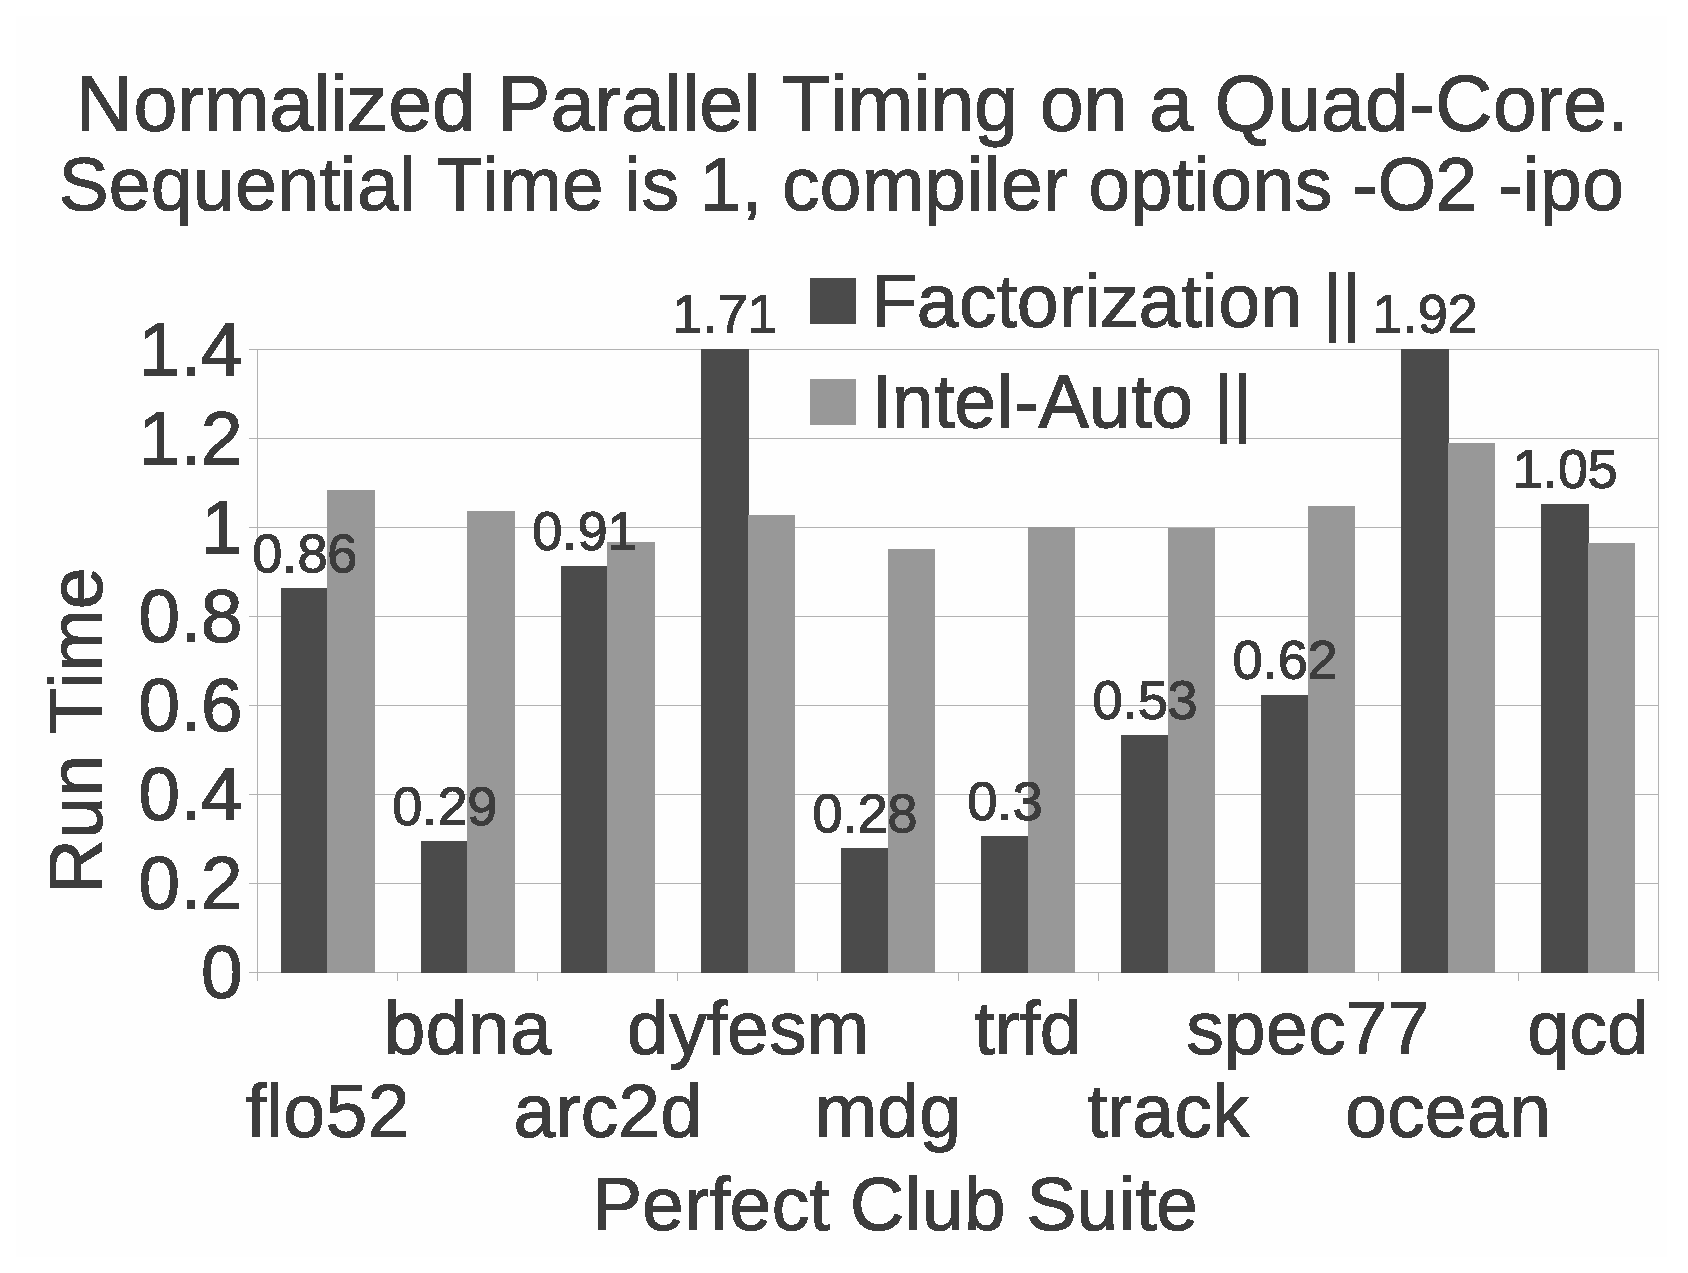
\includegraphics[height=22ex]{Figures/PerfectResO2}
\column{0.48\textwidth} 
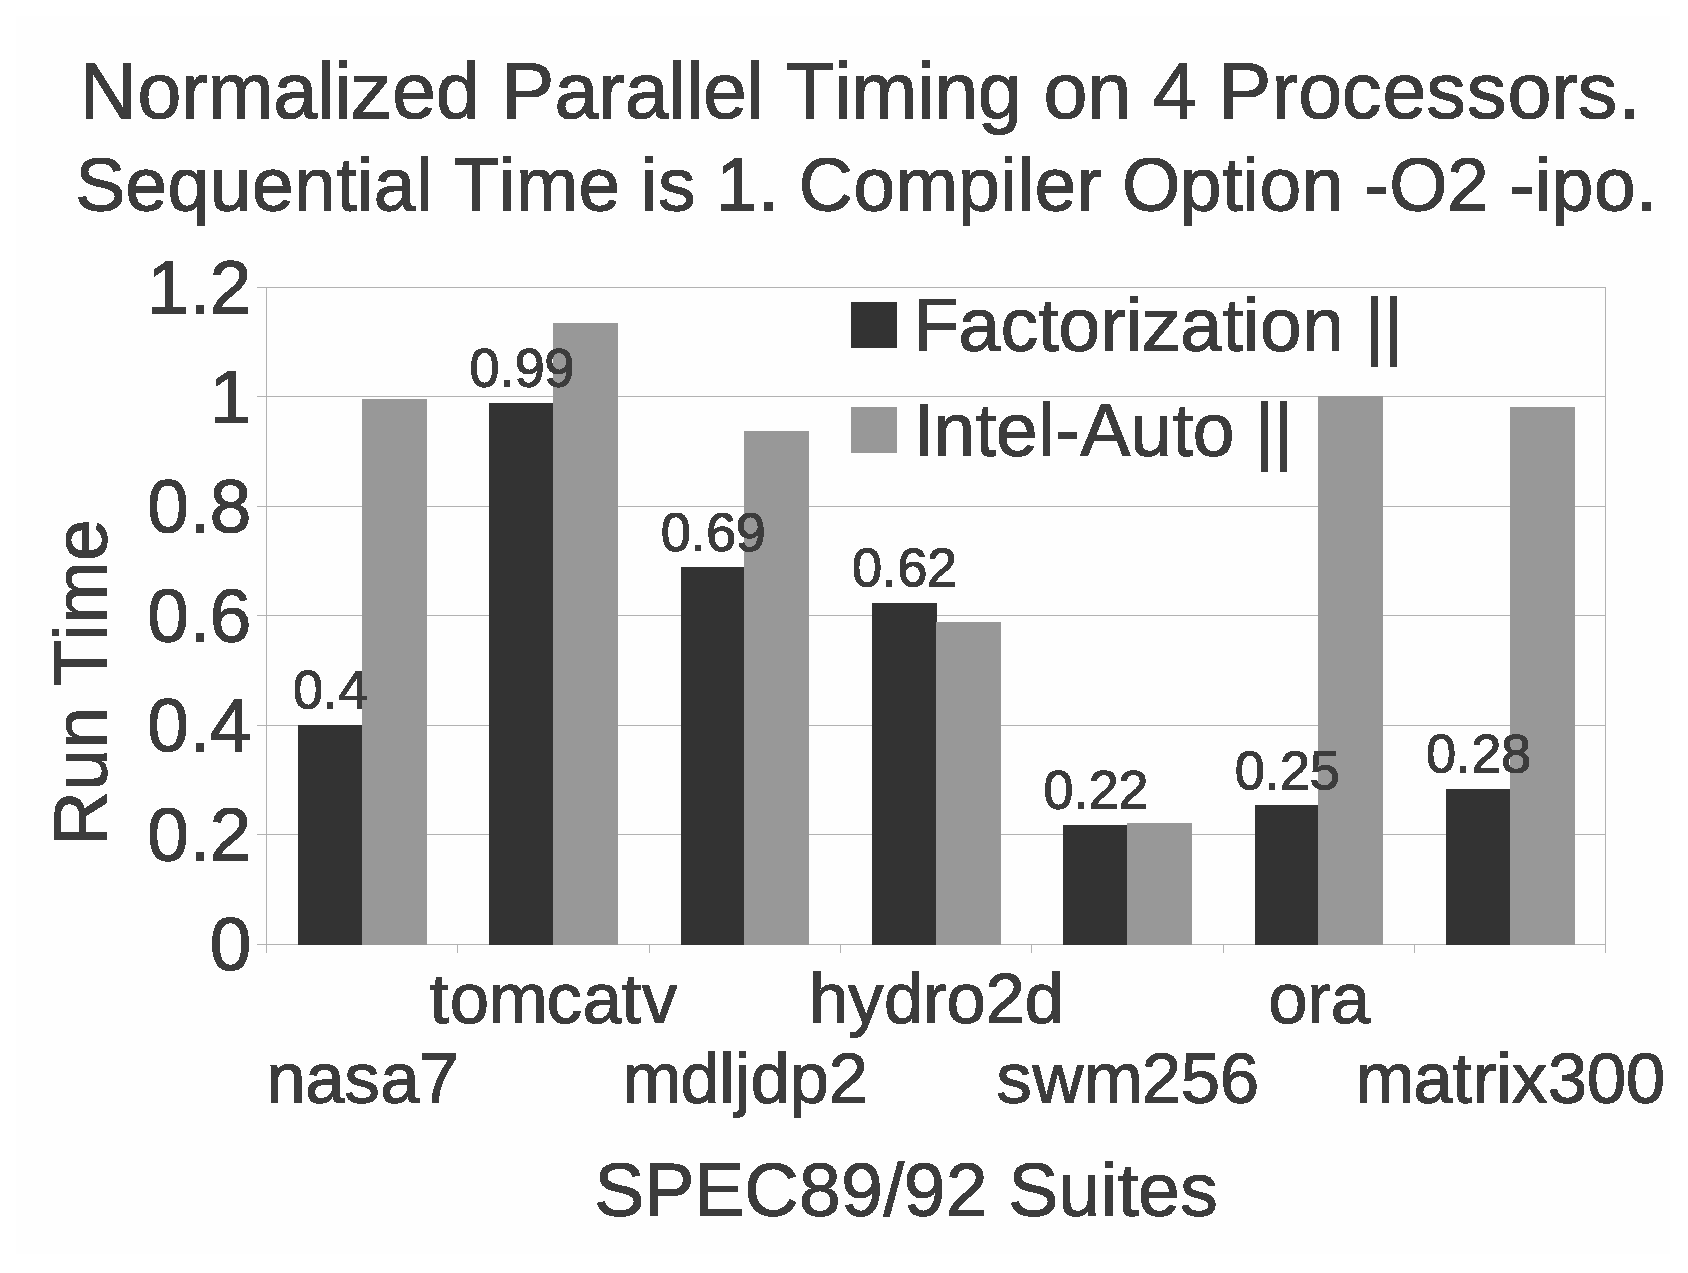
\includegraphics[height=22ex]{Figures/Spec92ResO2}
\end{columns}
%\smallskip
\begin{columns} 
\column{0.48\textwidth} 
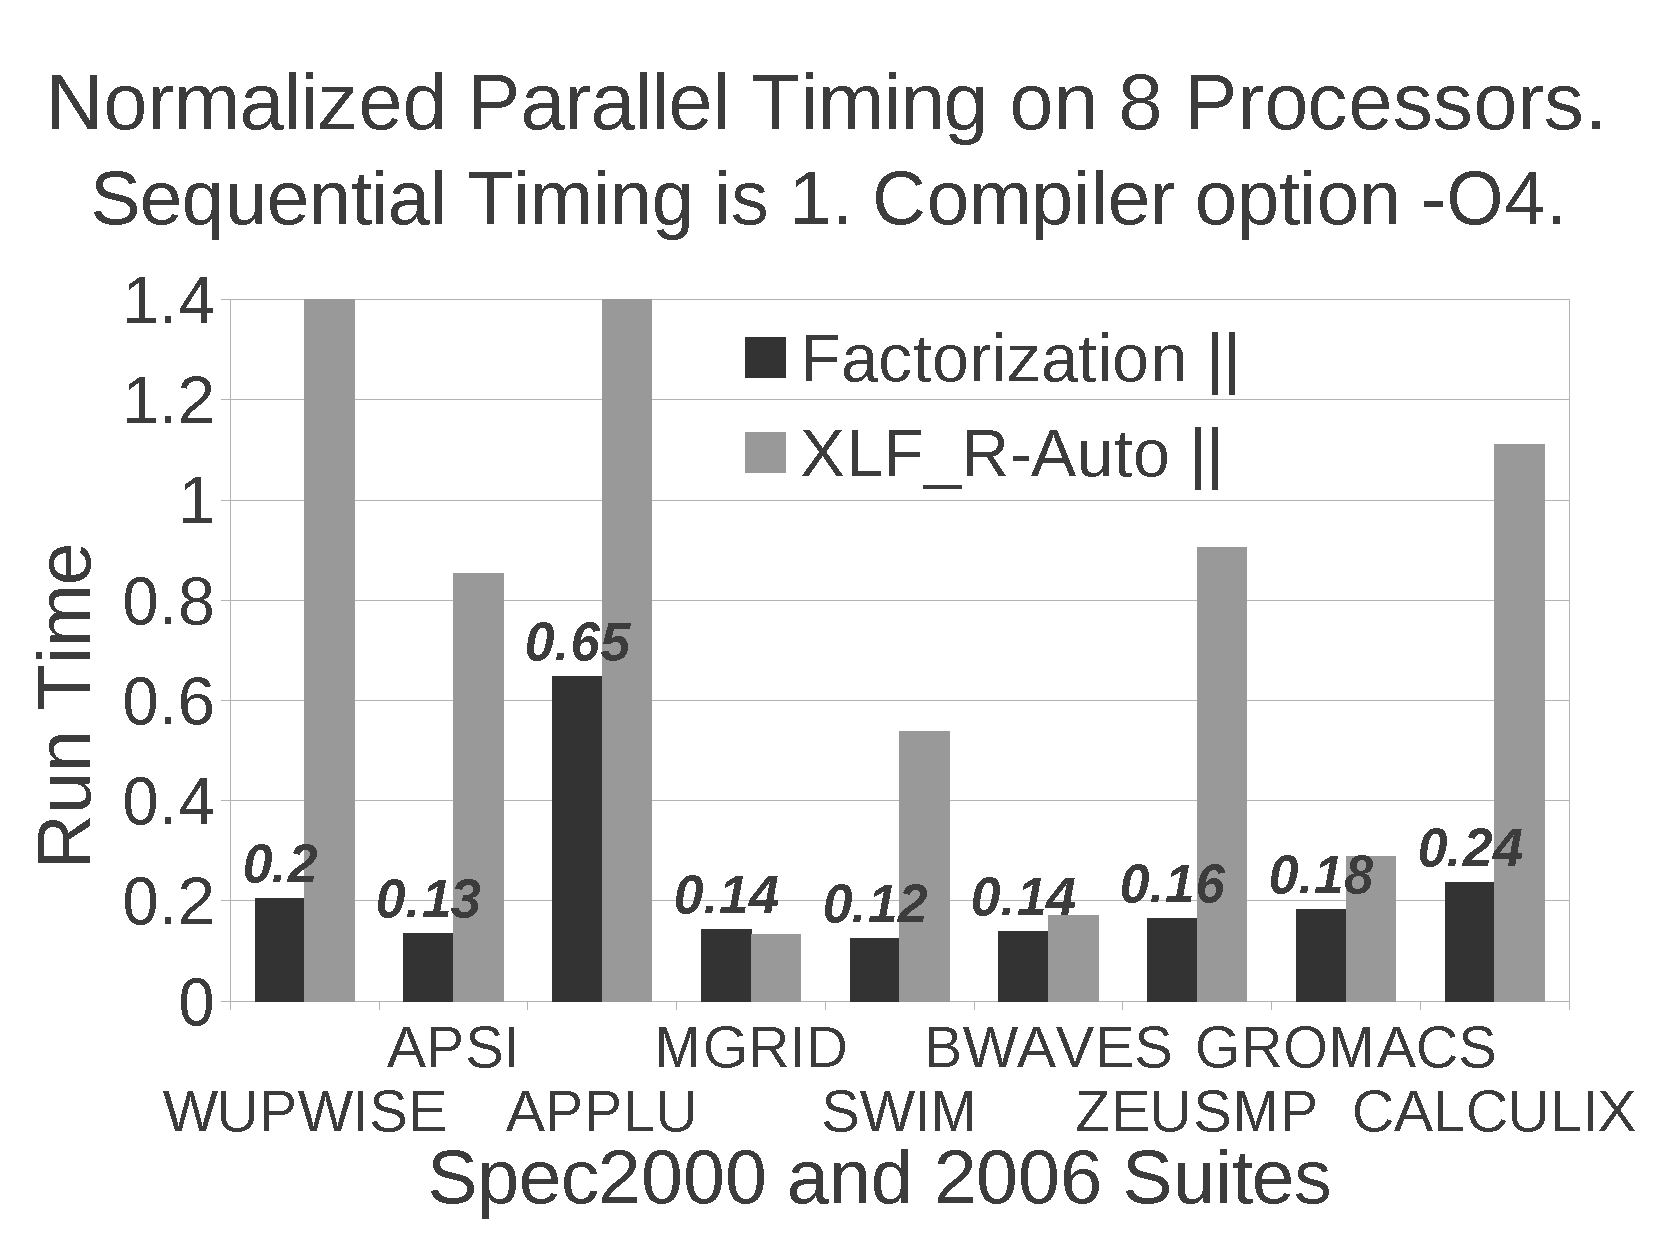
\includegraphics[height=25ex]{Figures/Spec2006Res}
\column{0.48\textwidth} 
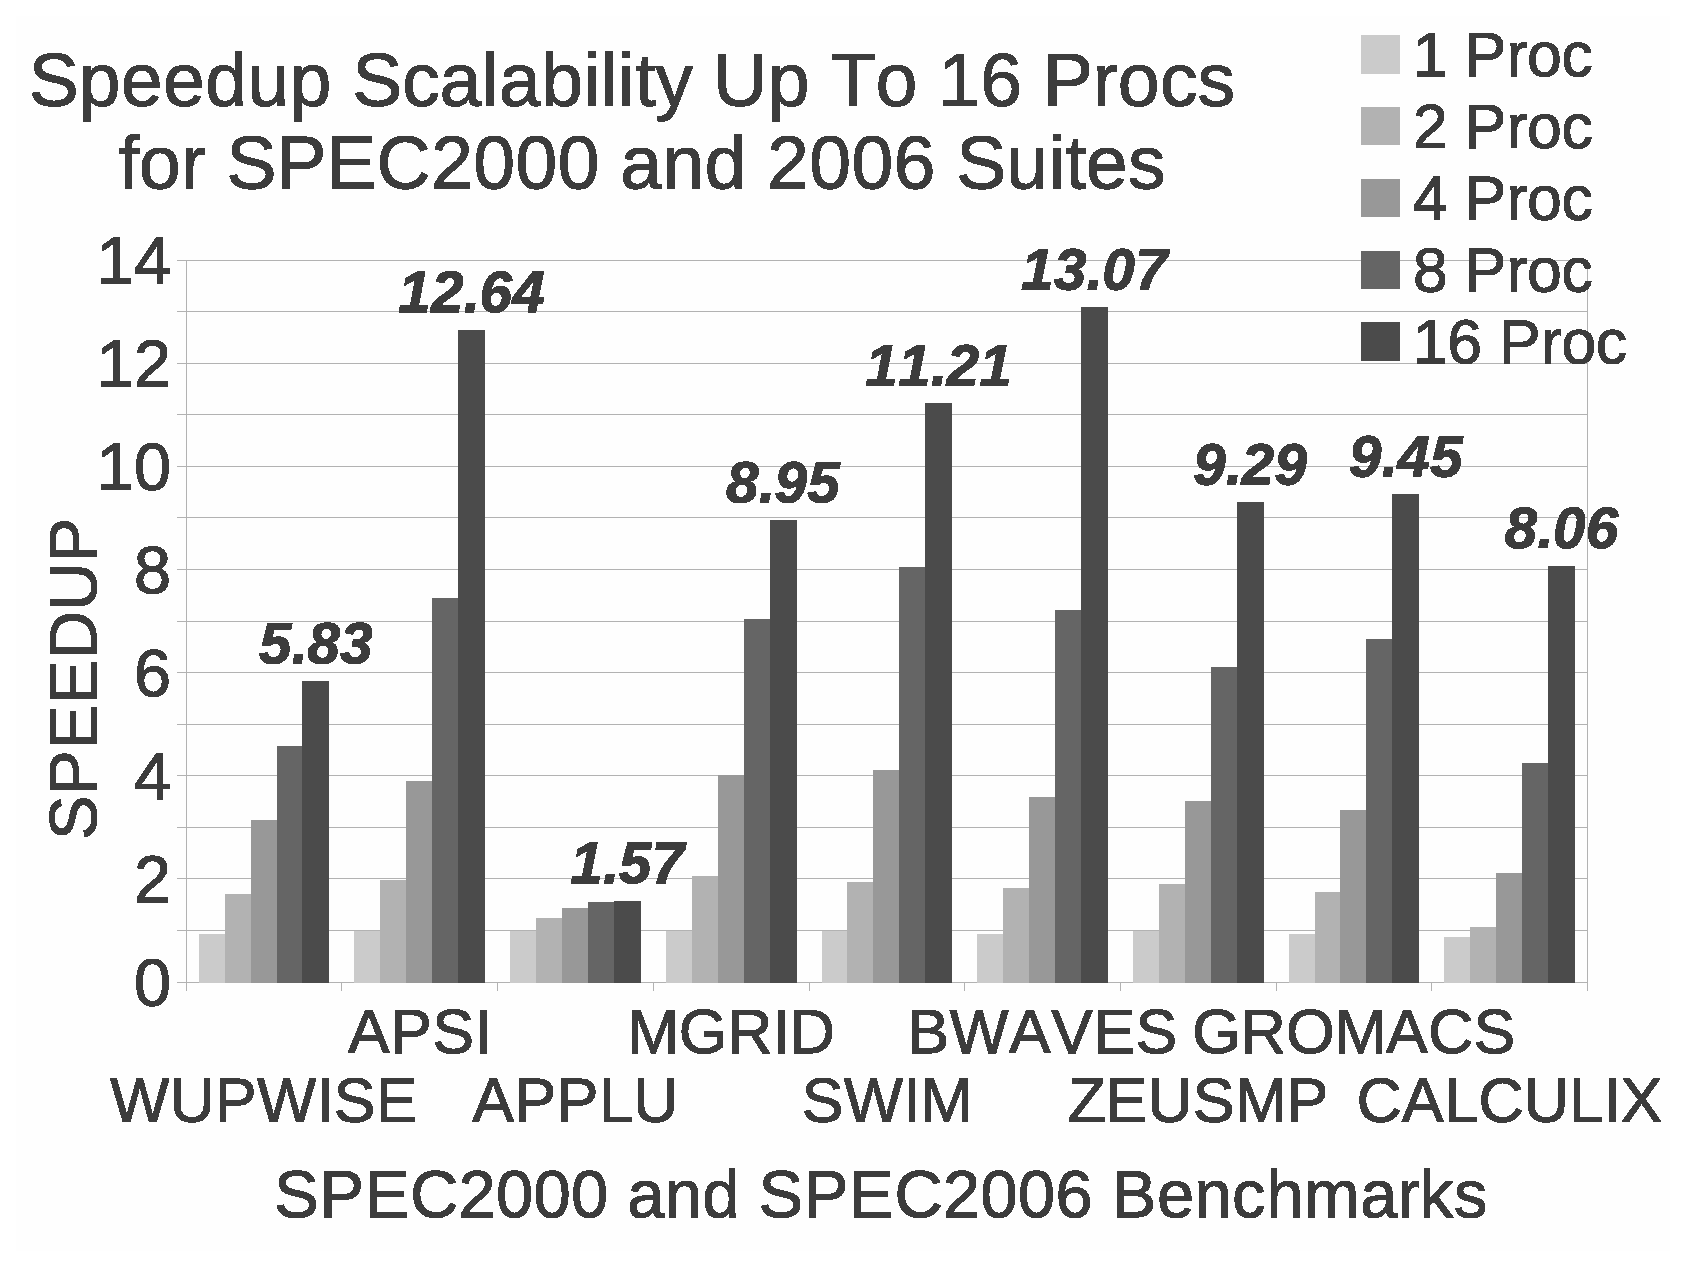
\includegraphics[height=25ex]{Figures/Spec2006SpeedupScalRTall}
\end{columns}

\end{frame}


\begin{frame}[fragile,t]
  \frametitle{Evaluation on $27$ {\sc perfect-club} \& {\sc spec} benches}
%  \frametitle{Paper's Approach Overview}

\emph{Analysis Is Effective in Most Cases:}\smallskip
\begin{itemize}
                \item Analyzed $2100$ loops, measured $380$ parallel loops $92\%$ runtime,\smallskip
                \item \emph{Good application-level speedup at negligible predicate overhead};
                        not pretty but effective, e.g., {\tt mafillsm\_do7} in {\scriptsize \textsc{Calculix}/\textsc{Spec2006}},\smallskip 
                \item \emph{Only 2 loops} out of 380, i.e., $\sim0.5\%$, \emph{require {\sc tls}}.
\end{itemize}

\bigskip
\pause
\emp{Sill a Heroic-Effort Solution:}\smallskip
\begin{itemize}
                \item \emp{Complex Analysis}: 2 {\em helper} {\sc ir}s \& optims, complex codegen\smallskip
                \item \emp{Compiler Magic}: parallelism may {\em not} be discovered, {\scriptsize 416.gamess}, 
                \item \emp{Main Difficulty}: user's optimizations obfuscates parallelism \& 
                  reverse engineering them is hard, e.g., {\tt scan} (prefix sum).\smallskip
                \item \emp{\bf Extraction of nested parallelism unfesible 
                            (many cores).}\medskip
\end{itemize}

%\alert{Obs:} Summary, Predicate, and SSA reps are pure functional langs!

{\tiny
%S.~Rus, L.~Rauchwerger and J.~Hoeflinger, ``Hybrid analysis: static \& dynamic memory reference analysis'', IJPP'03.
C.~E.~Oancea and L.~Rauchwerger, ''A Hybrid Approach to Proving Memory Reference Monotonicity'', LCPC'11.
C.~E.~Oancea and L.~Rauchwerger, ''Logical Inference Techniques for Loop Parallelization'', PLDI'12.$\mbox{\tt~~~~~~}$
C.~E.~Oancea and L.~Rauchwerger, ''Scalable Conditional Induction Variable (CIV) Analysis'', CGO'15.
}

%\includegraphics[height=7ex]{Figures/IND_PRED/indequ.ps}
%\includegraphics[height=7ex]{Figures/IND_PRED/pred_big.ps}
%\includegraphics[height=7ex]{Figures/IND_PRED/pred_o1.ps}

\end{frame}


\section{Auto Parallelization in Pure Functional Languages}

\begin{frame}[fragile]
	\tableofcontents[currentsection]
\end{frame}

\begin{frame}[fragile,t]
   \frametitle{Map-Reduce Functional Language}

\alert{Easier if parallelism is explicit map/reduce/scan ops \& nice algebra.}
\begin{itemize}
    \item also easier to reason when functions are math functions
    \item no destructive updates $\Rightarrow$ easier to extract inspectors (prg slices).
\end{itemize}
\bigskip

\emp{map} :: $((\alpha \rightarrow \beta), [\alpha]) \rightarrow [\beta] $ has \emph{\em inherently parallel semantics}.

\bigskip

\begin{tabular}{crcccccl}
x = & \emp{map}(~~~f, \{& $a_1$, & $a_2$, & .., & $a_n$ & \} & )\\
    &      & $\downarrow$ & $\downarrow$ &  & $\downarrow$ & &\\
x $\equiv$ &  \{  & \emph{f($a_1$)}, & \emph{f($a_2$)}, & .., & \emph{f($a_n$)} & \} &
\end{tabular}

\bigskip
\bigskip
\pause

\emp{Map Fusion:} (higher-order transformation)

\begin{tabular}{rccc}
a = & \{ $a_1$, $a_2$, .., $a_n$ \} & & a = \{ $a_1$, $a_2$, .., $a_n$ \} \\  
\emp{x =} & \emp{map( f, a )} & & \\
%  & $\downarrow$ & & \\
%//x = &  \{ \emph{f($a_1$)}, \emph{f($a_2$)}, .., \emph{f($a_n$)} \} & & \\
\emph{y} = & \emp{map( g, x )} & $\equiv$ & \emph{y} = \emp{map(g o f, a)}\\
  & $\downarrow$ & & \\
\emph{y} $\equiv$ &  \{\emph{g(f($a_1$))},\emph{g(f($a_2$))},..,\emph{g(f($a_n$))}\} & $\equiv$ & \{\emph{g(f($a_1$))},\emph{g(f($a_2$))},..,\emph{g(f($a_n$))}\} \\
\end{tabular}

\end{frame}


\begin{frame}[fragile,t]
   \frametitle{Map-Reduce Functional Language}

\bigskip

\emp{reduce} :: $((\alpha \rightarrow \alpha \rightarrow \alpha), \alpha, [\alpha]) \rightarrow \alpha$

\smallskip

\emp{reduce}($\odot$, $e$, \{$a_1$, $a_2$, ..., $a_n$\}) $\equiv$ \emph{$e \odot a_1 \odot a_2 \odot ... \odot a_n$}

\smallskip

~~~~~where $\odot$ is an associative binary operator.

\bigskip

\begin{center} 
        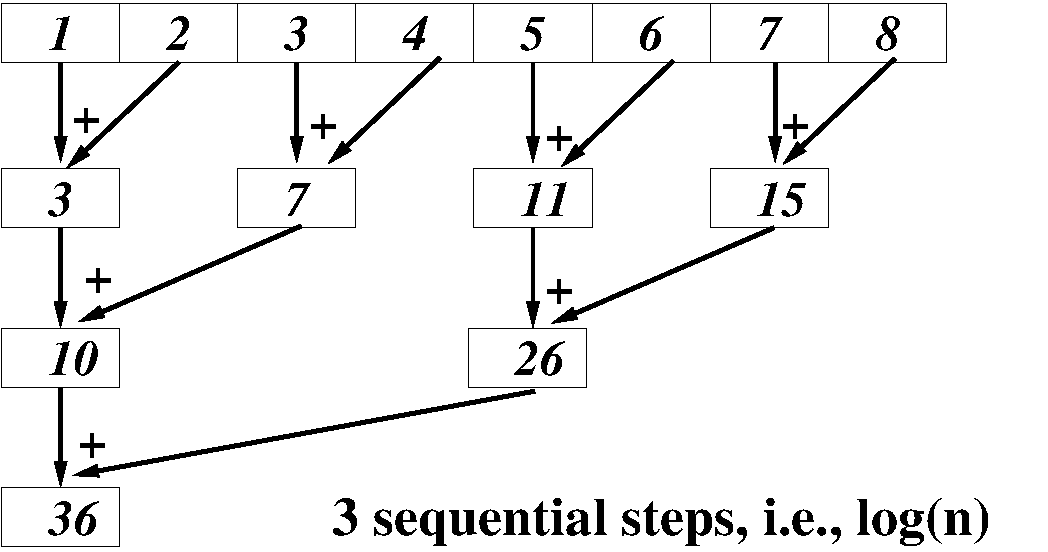
\includegraphics[height=18ex]{Figures/ReduceEg.pdf} 
\end{center}\bigskip

\emp{scan} :: $((\alpha \rightarrow \alpha \rightarrow \alpha), \alpha, [\alpha]) \rightarrow [\alpha]$

\smallskip

\emp{scan$^{exc}$}($\odot$, $e$, \{$a_1$, $a_2$, ..., $a_n$\}) $\equiv$ \emph{\{$e$, $e \odot a_1$, $\ldots$, $e \odot ... \odot a_{n-1}$\}}


Build programs by combining \emp{map}, \emp{reduce} and other such operators. %Example: \smallskip

\end{frame}


\begin{frame}
  \frametitle{List Homomorphisms $\equiv$ Map-Reduce Computation} 

\emp{List concatenation:} $++ : [\alpha] \rightarrow [\alpha] \rightarrow [\alpha]$\\
$[x_1, \ldots, x_k] ++ [x_{k+1}, \ldots, x_n] = [x_1, \ldots, x_n]$.

\smallskip

Observation: \emp{($[\alpha], ++$) monoid}, neutral element is the empty list.

\bigskip

\begin{mydef}[List Homomorphism]\label{ListHomDef}\vspace{-1ex}
$h :: [\alpha] \rightarrow \beta$ over finite lists is called a 
{\em list homomorphism} if there exists an associative binary operator 
$\odot :: \beta \rightarrow \beta \rightarrow \beta$, such that: \\
$\mbox{~~~~~~~~~~~~~~~~~~~~~~~}$
\emp{$h \mbox{ } (x{\tt ++}y) = (h\mbox{ }x)\mbox{ }\odot\mbox{ }(h\mbox{ }y)$} \\
\mbox{~~~~~~~~~~~~~~~~~~~~~~~~}\emp{$h\mbox{ }[x] = f\mbox{ }x$},\\
\mbox{~~~~~~~~~~~~~~~~~~~~~~~~}\emp{$h\mbox{ }[ ] = e_{\odot}$},\\
We denote a homomorphism $h$ by \emp{$h = hom \mbox{ }(\odot) \mbox{ }f\mbox{ }e_{\odot}$}.
\end{mydef}

\begin{mytheo}[1st List Homomorphism Theorem]\label{LHomLema}
\emp{$h~=~hom~(\odot)~f~e_{\odot}~~~\Leftrightarrow~~~h~=~(red~(\odot)~e_{\odot})~.~(map~f)$}
\end{mytheo}

\end{frame}


\begin{frame}[fragile,t]
  \frametitle{List Homomorphisms $\equiv$ Map-Reduce Computation}

\begin{mytheo}[1st List Homomorphism Theorem]\label{LHomLema}
\emp{$h~=~hom~(\odot)~f~e_{\odot}~~~\Leftrightarrow~~~h~=~(red~(\odot)~e_{\odot})~.~(map~f)$}
\end{mytheo}

\begin{block}{Examples of Map-Reduce}
\begin{columns}
\column{0.33\textwidth}\vspace{-2ex}
\begin{colorcode}[fontsize=\scriptsize]
\emph{len} :: [\mymath{\alpha}] -> Integer
\emph{len} []     = \emp{0}
\emph{len} [x]    = \emp{1}
\emph{len} (x++y) = (\emph{len} x) \emp{+} 
             (\emph{len} y)
\emp{len \mymath{\equiv} (red (+) 0) .}
       \emp{(map (fn x \mymath{\Rightarrow} 1))}
\end{colorcode}
\column{0.57\textwidth}\vspace{-2ex}
\begin{colorcode}[fontsize=\scriptsize]
-- logical and \emp{\mymath{\wedge}} :: \mymath{\alpha} -> \mymath{\alpha} -> Bool 
-- all elems satisfy p :: \mymath{\alpha} \mymath{\rightarrow} Bool ?
\emph{all\mymath{\myindx{p}}} :: [\mymath{\alpha}] -> Bool
\emph{all\mymath{\myindx{p}}} []     = \emp{True}
\emph{all\mymath{\myindx{p}}} [x]    = \emp{p x} 
\emph{all\mymath{\myindx{p}}} (x++y) = (\emph{all\mymath{\myindx{p}}} x) \emp{\mymath{\wedge}} (\emph{all\mymath{\myindx{p}}} y)
\emp{all\mymath{\myindx{p}} \mymath{\equiv} (red (\emp{\mymath{\wedge}}) True) .} \emp{(map (fn x \mymath{\Rightarrow} p x))}
\end{colorcode}
\end{columns}
\end{block}

%Cole: near homomorphism:
%given a list of integers, find the contiguous segment of the list 
%whose members have the largest sum among all such segments. 
%Return the sum (only).

\begin{block}{Maximum (Positive) Segment Sum Problem}
\begin{colorcode}
(mssx, misx, mcsx, tsx) \mymath{\odot} (mssy, misy, mcsy, tsy) = 
  ( (mssx\mymath{\mbox{ }\uparrow\mbox{ }}mssy\mymath{\mbox{ }\uparrow\mbox{ }}(mcsx+misy), misx\mymath{\mbox{ }\uparrow\mbox{ }}(tsx+misy), 
    (mcsx+tsy)\mymath{\mbox{ }\uparrow\mbox{ }}mcsy, tsx + tsy )
f x = (x\mymath{\mbox{ }\uparrow\mbox{ }}0, x\mymath{\mbox{ }\uparrow\mbox{ }}0, x\mymath{\mbox{ }\uparrow\mbox{ }}0, x)

\emph{mss = (red \mymath{\odot} (0,0,0,0)) . (map f)}
\end{colorcode}
\end{block}


\end{frame}


\begin{frame}[fragile,t]
  \frametitle{List Homomorphism Invariants}

%\begin{mytheo}[Map Fusion/Distribution]\label{Fusion}\vspace{-2ex}
%Given unary functions $f$ and $g$ then: \\
%$\mbox{ }\mbox{ }\mbox{ }\mbox{ }\mbox{ }\mbox{ }\mbox{ }\mbox{ }$
%$({\tt map}~f)~.~({\tt map}~g) \mbox{ }\mbox{ }\equiv\mbox{ }\mbox{ }{\tt map}~(f~{\tt{}.}~g)$ \\
%\end{mytheo}


\begin{mytheo}[List-Homomorphism Promotions]\label{LHomInv}\vspace{-2ex}
Given unary function $f$ and an associative binary operator $\odot$ then: \\
$\mbox{ }$ \\
1. $\mbox{ }\mbox{ }\mbox{ }\mbox{ }\mbox{ }\mbox{ }$
$({\tt map} \mbox{ }f)\mbox{ }.\mbox{ }({\tt red}\mbox{ }({\tt ++})) \mbox{ }\mbox{ }\equiv\mbox{ }\mbox{ }({\tt red}\mbox{ }({\tt ++}))\mbox{ }.\mbox{ }({\tt map}\mbox{ }({\tt map}\mbox{ }f) )$ \\
$\mbox{ }$ \\
2. $\mbox{ }\mbox{ }\mbox{ }\mbox{ }\mbox{ }\mbox{ }$
$({\tt red}\mbox{ }\odot)\mbox{ }.\mbox{ }({\tt red}\mbox{ }(++)) \mbox{ }\equiv\mbox{ }\mbox{ }({\tt red}\mbox{ }\odot)\mbox{ }.\mbox{ }({\tt map}\mbox{ }({\tt red}\mbox{ }\odot) )$
\end{mytheo}

\bigskip

Using {\tt distr}$_p :: [\alpha] \rightarrow [[\alpha]]$ to distribute the input list into $p$ sublists

\bigskip

\emp{{\tt (red $\odot$ $e_\odot$) . (map f)} $\equiv$} 
{\scriptsize {\tt (red $\odot$ $e_\odot$) . (map f) . \emph{id} $\equiv$}\\
{\tt (red~$\odot$~$e_\odot$) . \emph{(map~f) . (red~(++)~[])} . distr$_p~~\equiv$} \\
{\tt \emph{(red~$\odot$~$e_\odot$) . (red~(++)~[])} . (map~(map f)) . distr$_p~~\equiv$} \\
{\tt (red~$\odot$~$e_\odot$) . \emphh{map (red~(++)~[]) . (map~(map f))} . distr$_p~~\equiv$} }\\
\emp{{\tt (red~$\odot$~$e_\odot$)~.~(map ((red $\odot$ $e_\odot$)~.~(map f)))~.~distr$_p$}},

\end{frame}

\begin{frame}
  \frametitle{Flatenning: A Beautiful Transformation (Blelloch)}

    \begin{itemize}
        \item nested map-reduce parallelism on irregular arrays $\Rightarrow$
        \item flat map-reduce operations under \emphh{asymptotic work-depth guarantees}.\medskip

        \item suitable for a class of \emphh{divide and conquer algorithms}, 
                e.g., quicksort,\medskip

        \item \emp{often inneficient in practice}: does not optimize the common case, 
                (locality of reference, communication, efficient sequentialization).\medskip

%destroys the program structure.  
    \end{itemize}

\end{frame}


\section{Present Time: Searching for the Common Ground (Futhark)}

\begin{frame}[fragile]
	\tableofcontents[currentsection]
\end{frame}

\subsection{Motivation \& Problem Statement}

\begin{frame}
  \frametitle{Motivation}

Functional High-Performance Computing for Financial IT (HIPERFIT)
mathematical finance, programming languages, high-performance systems, 
and application experts from the financial sector. 
%
%simultaneous challenges of high transparency, high computational 
%performance and high productivity in finance

\bigskip\pause

\begin{itemize}

    \item Real-world financial programs: is there enough parallelism and can it be identified?\smallskip

    \item Capricious hardware, e.g., static parallelism, divergence, etc.\smallskip

    \item Can we actually get significant speedup on {\bf many cores}?\smallskip

    \item Is this beyond the common user? How tedious is it?\bigskip

\end  {itemize}
\pause

\emp{\em Our journey to answer these questions started with ... \\
            the real-world code from our beloved industry partners.}\bigskip

\emphh{\em And motivated the design of a language, named Futhark,\\
        and its optimizing compiler -- work in progress.}

\end{frame}

\begin{frame}
  \frametitle{Why Language?}

Are there not many enough already? {\sc cuda}, \textsc{OpenCL}, {\sc mpi}.\smallskip

Rumor is \emp{\em industry unwilling to rewrite codebase ...\pause more than once.}\smallskip

Such solutions $\Rightarrow$ unmaintainable code (far away from the algorithm),\\
$\mbox{\tt~~~~~~~~~~~~$\Rightarrow$~}$timestamped for a given hardware/dataset. 
\bigskip

Findings: there seems to be

\begin{itemize}

    \item a lot of available parallelism ... some more visible than other\smallskip

    \item small set of parallel basic blocks:
            map, reduce, filter, scan, etc.,\smallskip

    \item but not necessarily easy to exploit:\bigskip\pause

    \item \emphh{\em Rich composition of nested parallelism in nontrivial control flow,}\smallskip

    \item \emp{\em with the occasional awfully dependent loop}.\smallskip

\end{itemize}

\emphh{Need to specify all available parallelism \&\\ 
        the way in which it can be (de)composed.}

\end{frame}


\begin{frame}[fragile,t]
  \frametitle{Why Optimizing Compiler?}

\begin{itemize}
    \item Significant speedups can be achieved, but 

    \item tedious transformations, which often requires specialist users!

    \item \emp{\em Challenge: ``one size does NOT fit all''} \smallskip

    \item Speedup differs significantly between applications,

    \item and between different datasets of the same application.\smallskip

    \item \emphh{\em Efficient parallelization is sensitive to the dataset}
        \begin{itemize}
            \item e.g., degree of parallelism, memory footprint.
            \item Tradeoffs: fusion vs fission,
            \item parallelization {\em vs} efficient sequentialization.
        \end{itemize}

\end{itemize}

Expressiveness and Efficiency: requires both imperative \& functional constructs and optimizations! 

\smallskip

\tiny{C.~Oancea et. al., ``Financial software on GPUs: between Haskell and Fortran'', FHPC'12.\\
T.~Henriksen and C.~Oancea, ``A T2 Graph-Reduction Approach To Fusion'', FHPC'13.\\
T.~Henriksen, M.~Elsman and C.~Oancea. ``Size Slicing - A Hybrid Approach to Size Inference in Futhark'', FHPC'14.\\
T.~Henriksen and C.~Oancea. ``Bounds Checking: An Instance of Hybrid Analysis'', Array'14.\\
C.~Oancea, et. al., ``A Financial Benchmark for GPGPU Compilation'', CPC'15.
}


\end{frame}


\subsection{Option Pricing Benchmark}

\begin{frame}[fragile]
	\tableofcontents[currentsubsection]
\end{frame}

\begin{frame}[fragile,t]
\frametitle{Close to the Algorithm: Option Pricing in Futhark}

\emp{Contract Example}: You receive 100\$ next month and you return 95\$ in one 
year time plus the absolute difference between stocks (underlyings) $X_1$ and $X_2$ at 
dates $D_1$ and $D_2$.  \emp{What is the price of this contract NOW?} 


\begin{center}
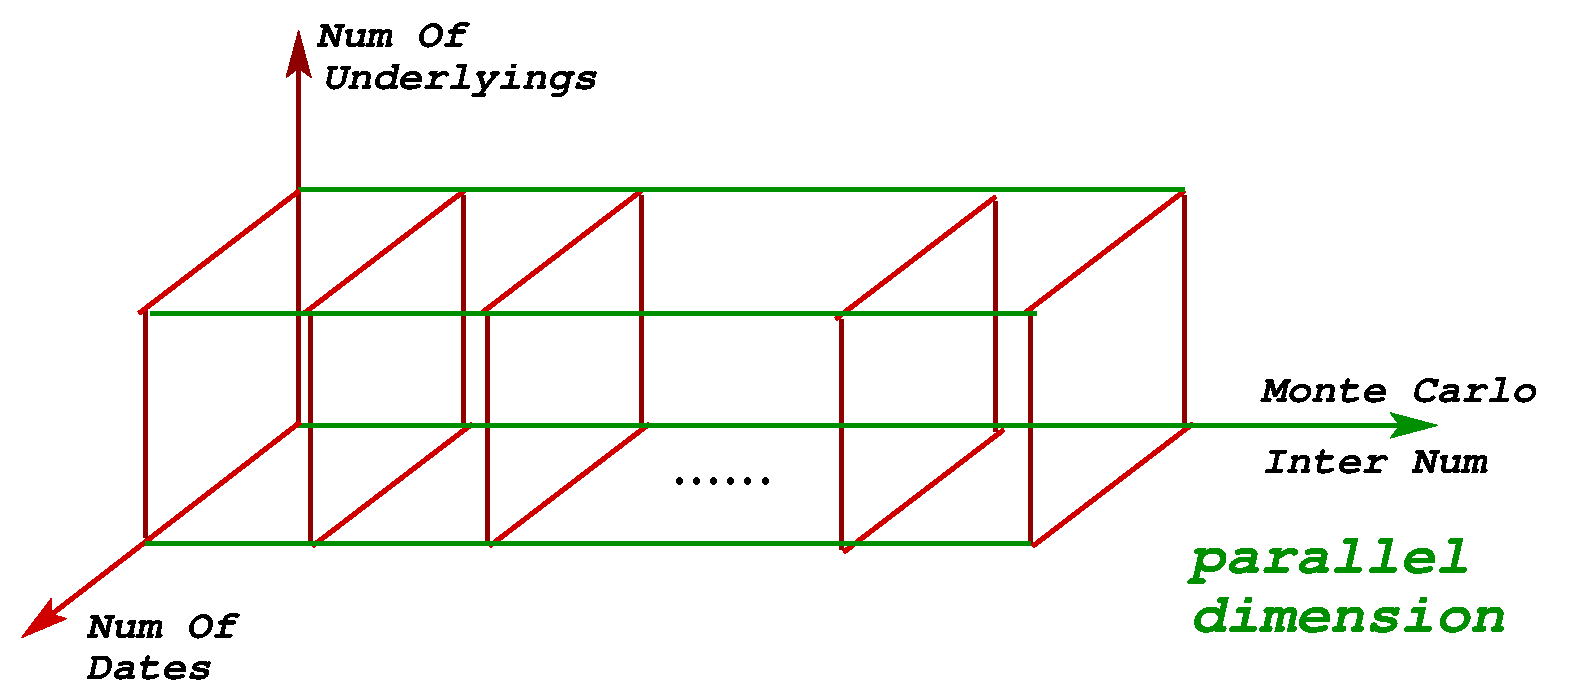
\includegraphics[height=18ex]{Figures/PricingMemSpace}
\end{center}

\begin {itemize}
    \item Generate independent Sobol sequences (uniform in $[0,1)$ ) % random numbers)
    \item Transform into Gaussian distribution $ ( -\infty , \infty )$ (numerical $\int$~)
    \item Brownian bridge for all dates, for each underlying
    \item Compute trajectories using Black-Scholes
    \item Monte-Carlo aggregation with product's payoff and discount
\end{itemize}
\end{frame}

\begin{frame}[fragile,t]
  \frametitle{Staying Close to the Algorithm: Option Pricing}

\begin{colorcode}
fun \emphh{[real]} mcPricing( //\emphh{\mymath{\mymathbb{R}\myindu{m}}} 
        int n, int d, int u, int m, int contract, int sob_bits, 
        [[int ]] sob_dirs,   ([[int ]], [[real]])     bb_data, 
        \blue{[( [[real]], [[real]], [[real]], [real] )]}    md_blsch,
        \blue{[( [real], [real] )]}                          md_payof) =

  let \emp{prices} = \emphh{map} (                                          //\emp{\mymath{\mymathbb{R}\myindu{n\times{}m}}}
      \emp{fn [int] (int sn)} =>                                    //\emp{\mymath{\mymathbb{N}\rightarrow\mymathbb{R}\myindu{m}}}
            let num = sn + 1 in
         in let \emp{sob} = sobolIndR(sob_bits,sob_dirs,\emp{num})        //\emp{\mymath{\mymathbb{Z}\rightarrow[0,1)\myindu{u\cdot{}d}}}
         in let \emp{gau} = ugaussian(\emp{sob})                          //\emp{\mymath{[0,1)\myindu{u\cdot{}d} \rightarrow \mymathbb{R}\myindu{u\cdot{}d}}}
         in let \emp{bbr} = brownBridge(u,d,bb_data,\emp{gau})            //\emp{\mymath{\mymathbb{R}\myindu{u\cdot{}d}\rightarrow\mymathbb{R}\myindu{u\times{}d}}}
         in let \emp{bsh} = \emphh{map}(blackScholes(u,bbr), \blue{md_blsch})      //\emp{\mymath{\mymathbb{R}\myindu{m\times{}u\times{}d}}}
         in let \emp{pay} = \emphh{zipWith}(payoff(contract), bsh,\blue{md_payof}) //\emp{\mymath{\mymathbb{R}\myindu{m}}}
            in        \emphh{map}( op /(toReal(n)), pay)              //\emp{\mymath{\mymathbb{R}\myindu{m}}}  
    , \emp{iota(n)} ) //\emp{\{0\mymath{\ldots}n-1\}\mymath{\in\mymathbb{Z}\myindu{n}}} 

  in \emphh{reduce}(zipWith(op +), replicate(m,0.0), \emp{price})           //\mymath{\emp{\mymathbb{R}\myindu{n\times{}m}}\rightarrow\emphh{\mymathbb{R}\myindu{m}}}
\end{colorcode}
\bigskip 

\emphh{\bf Fusion {\em vs} Fission.}

\end{frame}


\begin{frame}[fragile,t]
  \frametitle{Sobol Component of Option Pricing}

There is outer parallelism and also some extra inner parallelism.\bigskip

\begin{itemize}
    \item Sobol Independent formula: $x_i = \bigoplus_{k \geq 0} B(i)_k \cdot m_k$,\bigskip
%    \item Sobol Recurrent   formula: $x_{i+1} = x_{i} \oplus m_c$, where $c$ pos of lszb(i).  
%    \item Sobol sequence $\Rightarrow$ $s$-ary zipping of Sobol seq for $1$-dim values...
\end{itemize}

\begin{colorcode}
fun int  grayCode(int x) = (x >> 1) ^ x \blue{// ^ denotes xor, \& bitwise and} 
fun bool testBit(int n, int ind) = let t = (1 << ind) in (n & t) == t 

\blue{// Sobol Independent Formula;} sob_dirs \mymath{\in \mathbb{N}\myindu{(u\cdot{}d)\times{}num_bits}}
fun [int] sobolInd(int bits_num,[[int]] sob_dirs,int i)=
   let inds = \emphh{filter}(testBit(grayCode(i)), iota(num_bits))
   in         \emphh{map}( fn int ([int] dir_vct) => 
                       let row = \emphh{map}(fn int(int i)=>dir_vct[i], inds )
                       in     \emphh{reduce}( op ^, 0, row )
                 , sob_dirs )

//the first n Sobol sequences can be computed with:
//\emphh{map( sobolInd(num_bits,sob_dirs), [0..n-1] )}
\end{colorcode}
\smallskip

\begin{itemize}
    \item \emphh{$O(1)$-depth parallelism}, but \emp{expensive work}. 
\end{itemize}


\end{frame}


\begin{frame}[fragile,t]
  \frametitle{Sobol Component of Option Pricing}

\begin{itemize}
%    \item Sobol Independent formula: $x_i = \bigoplus_{k \geq 0} B(i)_k \cdot m_k$,\smallskip
    \item Sobol Recurrent   formula: $x_{i+1} = x_{i} \oplus m_c$,\\ 
            where $c$ is the position of the least significant zero bit of $B(i)$.\bigskip
%    \item Sobol sequence $\Rightarrow$ $s$-ary zipping of Sobol seq for $1$-dim values...
\end{itemize}


\begin{colorcode}
\blue{// Sobol Strength-Reduced (Recurrent) Formula}
fun [int] sobolRec([[int]] sob_dirs, [int] prev, int i)=
        let col = \emp{recM}(sob_dirs, i) in \emphh{zipWith}(op^,prev,col)

fun [int] \emp{recM}( [[int]] sob_dirs, int i ) =
        let bit= index_of_least_significant_0(i) in
        \emphh{map}( fn int([int] row) => row[bit], sob_dirs )

//the first n Sobol sequences can be computed with:
//\emp{(scan( zipWith(op^), [0..0], map( recM(sobol_dirs), [1..n]))}
\end{colorcode}
\smallskip

\begin{itemize}
    \item \emphh{Less sequential work}, but \emp{$O(lg~n)$-depth parallelism}. \bigskip
\end{itemize}

Independent {\em vs} Strength Reduction Formulas $\equiv$\\
Degree of Parallelism {\em vs} Efficient Sequentialization. 

\end{frame}



\begin{frame}[fragile,t]
  \frametitle{Brownian Bridge: Imperative-Like Code}

\begin{itemize}
    \item Imperative features: {\tt do} loop \& in-place updates,\\
            e.g., to express sequential computation.\bigskip
\end{itemize}

%fun [[real]] brownBridge (int u, int d, ([[int]],[[real]]) bb_data, [real] gauss) =
%  \blue{bb_inds \mymath{\in \mymathbb{N}\myindu{3\times{}d}}, bb_coef \mymath{\in \mymathbb{R}\myindu{3\times{}d}}, gauss\mymath{\in \mymathbb{R}\myindu{d\cdot{}u}}}
%  let (bb_inds,bb_coef) = bb_data in
%  let (bi, li, ri) = (bb_inds[0], bb_inds[1], bb_inds[2]) in
%  let (sd, lw, rw) = (bb_coef[0], bb_coef[1], bb_coef[2]) in


\begin{colorcode}
  \emphh{map( fn [real] ([real] gau) => } \blue{// \mymath{\lambda :: \in \mymathbb{R}\myindu{d}\rightarrow \mymathbb{R}\myindu{d}}}
         let res = copy( replicate(d, 0.0) )   in
         let res[ bi[0] - 1 ] = sd[0] * gau[0] in

         \emp{loop(res) = for i < d-1 do}
           let (j,k,l) = (li[i+1]-1, ri[i+1]-1,bi[i+1]-1) in

           let tmp = \emp{res[k]}*rw[i+1] + sd[i+1]*gau[i+1]   in

           let \emp{res[l] =} if( (j + 1) == 0) then tmp
                        else tmp + lw[i+1] * \emp{res[j]}
           in  res
         in res
     \emphh{, transpose( reshape((d,u), gauss)) )}\blue{//map result \mymath{\in\mymathbb{R}\myindu{u\times{}d}}}
\end{colorcode}
\smallskip

\begin{itemize}
    \item Each element of {\tt res} is produced from two other elements of 
            statically-unknown index, produced in some previous iterations. 
    \item Parallel (map) and Sequential (loop) code can be combined. \bigskip
\end{itemize}

\end{frame}

\begin{frame}[fragile,t]
    \frametitle{Hardware and Datasets}

H1: Intel 7 System, 16 cores  Xeon(E5-2650 v2) 2-way MT \@2.6GHz \&\\
$\mbox{ }~~~~$GeForce GTX 780 Ti NVIDIA GPGPU 3Gbytes, 2880 cores @1.08.\\\smallskip

H2: AMD Opteron system, 32 cores (6274) @2.2 GHz \&\\
$\mbox{ }~~~~$GeForce GTX 680 NVIDIA GPGPU 2Gbytes, 1536 cores @1.02.\\\bigskip

Small: $u\times d$ = $1\times 1$\\
Medium: $u\times d$ = $3\times 5$\\
Large: $u\times d$ = $3\times 365$

\end{frame}



\begin{frame}[fragile,t]
\frametitle{Option Pricing Evaluation}

\emp{We measure hand-tuned {\sc gpgpu} code.}

H1 CPU Sequential: 0.8,   1.28, 11.23 seconds\\
H2 CPU Sequential: 1.54,  2.14, 16.06 seconds

\smallskip

\begin{columns}
\column{0.48\textwidth}
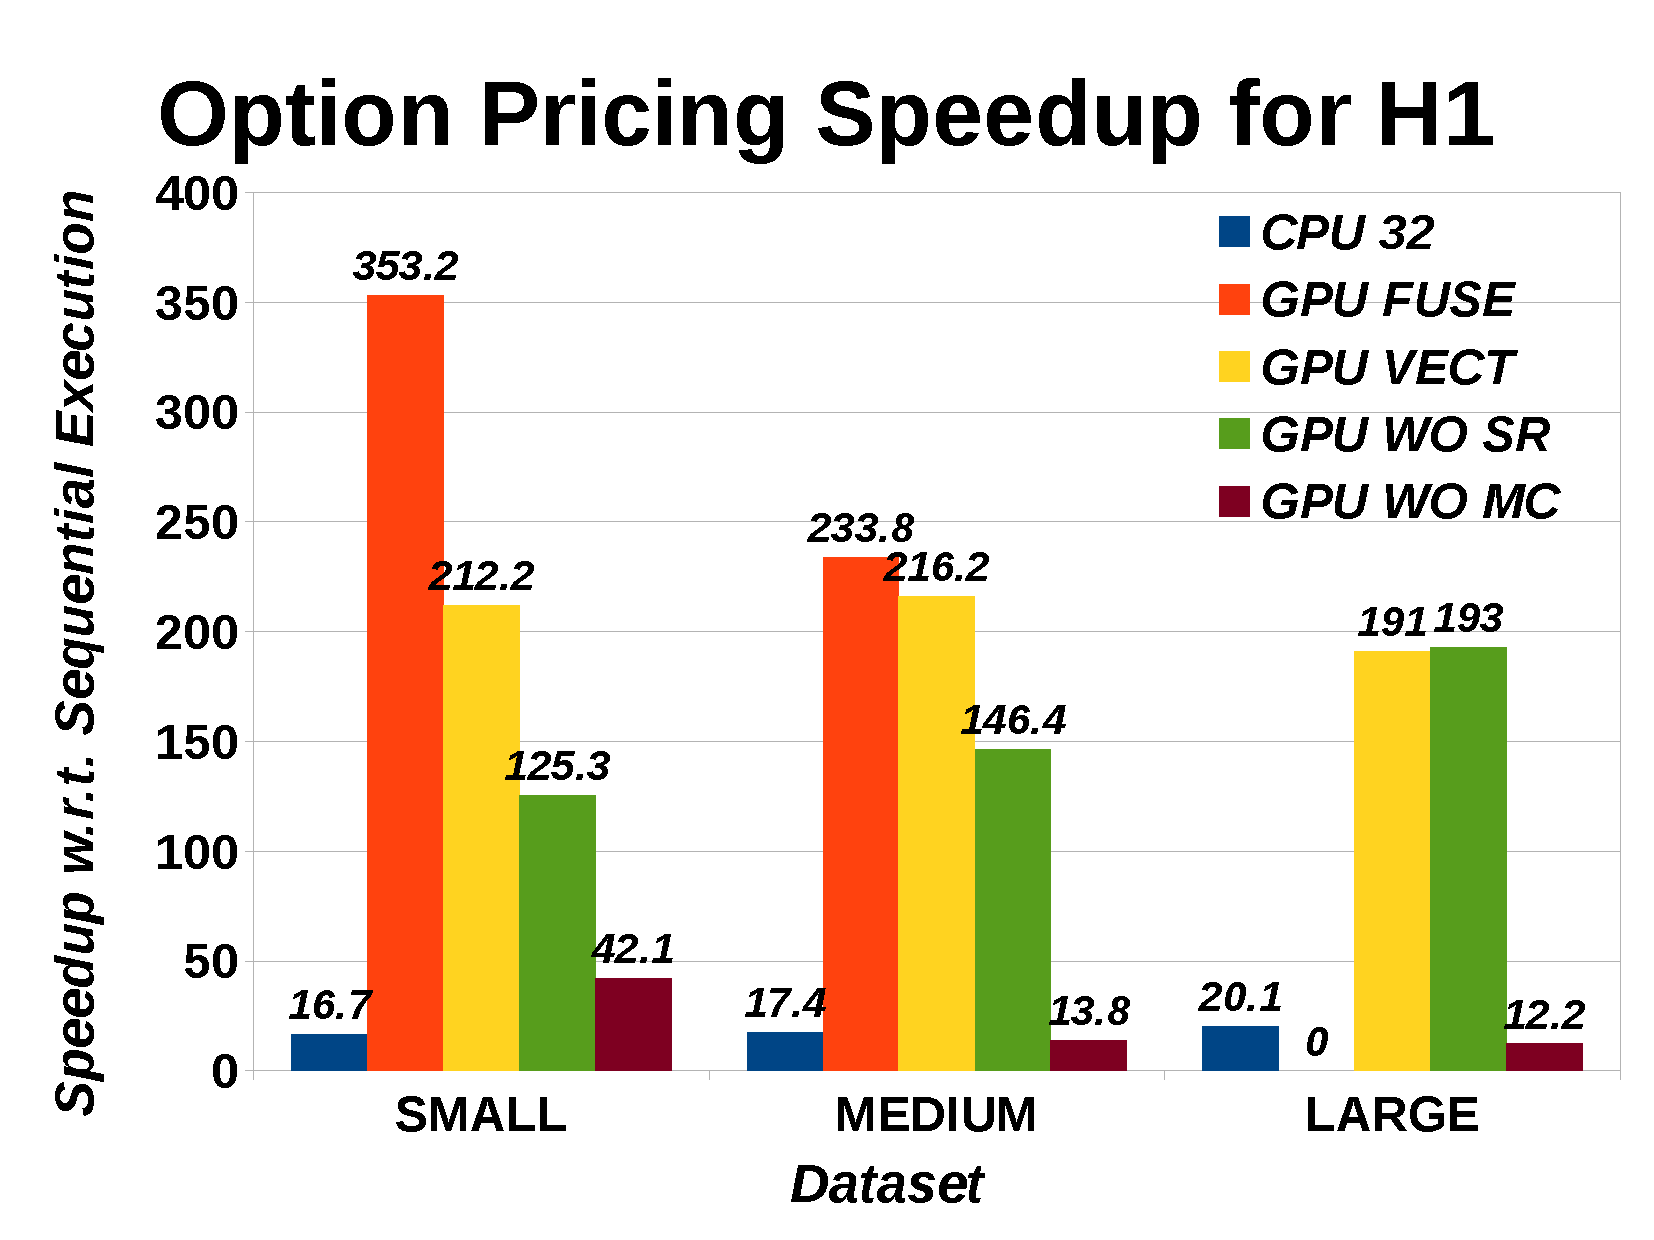
\includegraphics[height=27ex]{Figures/OptionPricing.pdf} 
\column{0.48\textwidth}
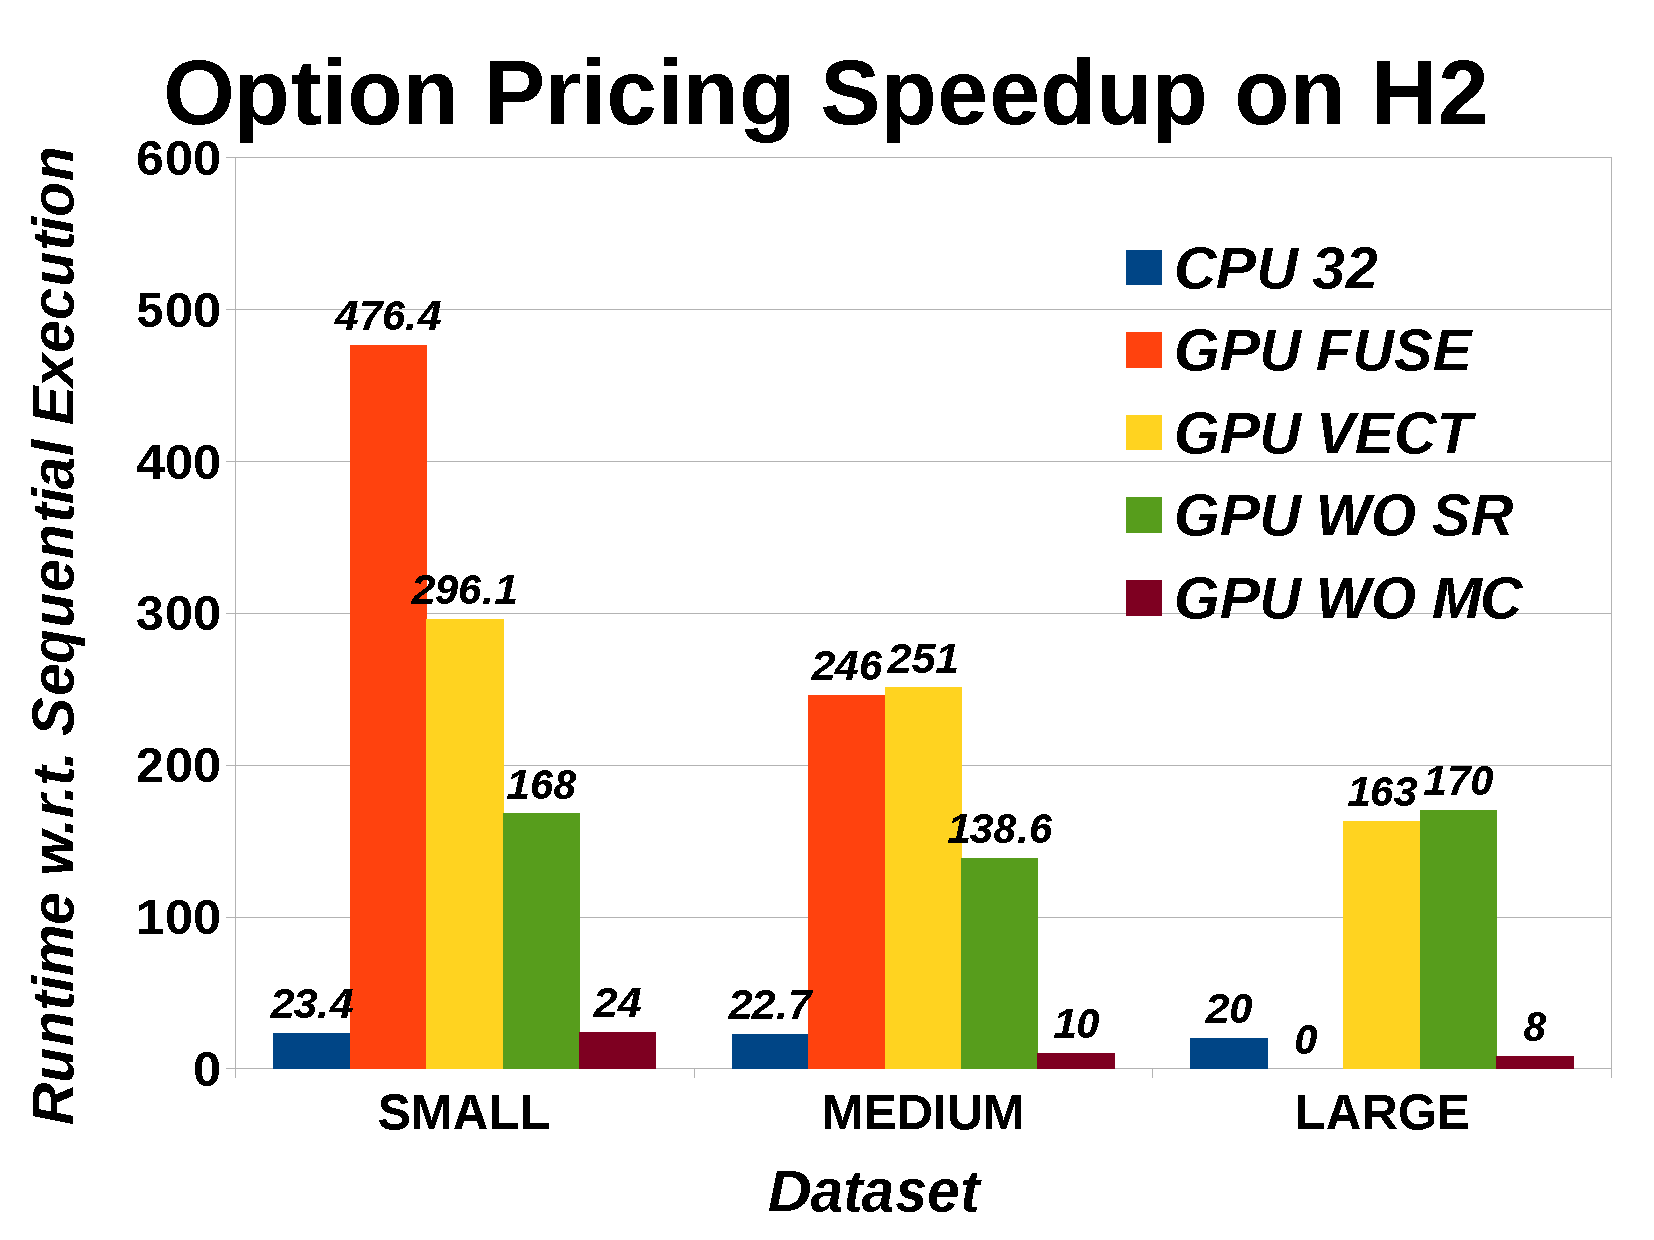
\includegraphics[height=27ex]{Figures/OptionPriceResNapo.pdf} 
\end{columns}
\end{frame}


%%%%%%%%%%%%%%%%%%%%%%%%%%%%%%%%%%%%%%%%

\subsection{Volatility Calibration Benchmark}

\begin{frame}[fragile]
	\tableofcontents[currentsubsection]
\end{frame}

\begin{frame}[fragile,t]
\frametitle{Market Calibration: Problem Statement}

\emp{\em Stochastic Volatility Calibration}: given a set of (observed) 
prices of contracts, identify a model of such prices, as
a function of volatility (unknown), time and strikes (known),
and some other (unobserved) parameters.
%and unobserved parameters like alpha, beta, nu, etc.

\bigskip

Volatility is modeled as a system of continuous partial differential
equations and solved via Crank-Nicolson finite-difference method:


\begin{equation}
\frac{\partial f}{\partial t}(x,t)\mbox{ }+\mbox{ }\mu(x,t)\frac{\partial f}{\partial x}(x,t)\mbox{ }+\mbox{ }
\frac{1}{2}\sigma(x,t)^{2}\frac{\partial^{2} f}{\partial x^{2}}(x,t)\mbox{ }-\mbox{ }
r(x,t)f(x,t) = 0
\end{equation}

\bigskip

\emp{It comes down to solving this equation for many instances of $\mu, \sigma, r$.}

\end{frame}

\begin{frame}[fragile,t]
\frametitle{Market Calibration: Multi-Core Parallelization}


\begin{block}{OpenMP Pragma for the Outermost Parallel Loop}
\begin{columns}
\column{0.48\textwidth}
\begin{colorcode}
\emp{REAL strike;}
\emp{PrivGlobs globs(numX,numY,numT);}

\emp{for(int i=0; i<outer; ++ i)} \{
  strike = 0.001*i;
  res[i] = value( globs,s0,strike,t,
                  alpha,nu,   beta,
                  numX, numY, numT );
\}
\end{colorcode}
\column{0.51\textwidth}
\begin{colorcode}
\emphh{\#pragma omp parallel for schedule(static)}
for(int i=0; i<outer; ++ i) \{
  \emphh{REAL strike;}
  \emphh{PrivGlobs globs(numX,numY,numT);}
  strike = 0.001*i;
  res[i] = value( globs,s0,strike,t,
                  alpha,nu,    beta,
                  numX, numY,  numT );
\}
\end{colorcode}
\end{columns}
\end{block} 
\bigskip

Not so bad: moves two lines and adds a \textsc{OpenMP} pragma.\bigskip

How difficult can {\sc gpu} parallelization be?\\
\emp{\bf Project for the PMPH Master Course.}

\end{frame}



\begin{frame}[fragile,t]
  \frametitle{Reasoning About Parallelism: Privatization} % of CPU, Multicores, GPGPU

If every array read is covered by a previous write in the same iteration\\
$\Rightarrow$ privatization is safe.\bigskip

\begin{columns}
\column{0.47\textwidth}
\begin{colorcode}
\emp{float A[N];}
\emp{for(int i=0;i<M;i++)\{ //seq}
  for(int j=0;j<N;j++)\{
    A[j] = ...
  \}
  ...
  for(int j=0;j<N;j++)\{
    ... = A[j]
  \}  
\}
\end{colorcode}
\column{0.47\textwidth}
\begin{colorcode}
\emphh{for(int i=0;i<M;i++)\{ //par}
  \emphh{float A[N];}
  for(int j=0;j<N;j++)\{
    A[j] = ...
  \}
  ...
  for(int j=0;j<N;j++)\{
    ... = A[j]
  \}  
\}
\end{colorcode}
\end{columns}

\end{frame}

\begin{frame}[fragile,t]
  \frametitle{Array Expansion} % of CPU, Multicores, GPGPU

No dynamic allocation on {\sc gpu} \& array {\tt N} is dataset specific.\smallskip

\begin{block}{Semantically Equivalent: Privatized {\em vs} Expanded {\tt A}}
\begin{columns}
\column{0.47\textwidth}
\begin{colorcode}
\emphh{for(int i=0;i<M;i++)\{ //par}
  \emp{float A[N];}
  for(int j=0;j<N;j++)\{
    \emp{A[j]} = ...
  \}
  ...
  for(int j=0;j<N;j++)\{
    ... = \emp{A[j]}
  \}  
\}
\end{colorcode}
\column{0.47\textwidth}
\begin{colorcode}
\emphh{float A[M, N];}
\emphh{for(int i=0;i<M;i++)\{ //par}
  for(int j=0;j<N;j++)\{
    \emphh{A[i,j]} = ...
  \}
  ...
  for(int j=0;j<N;j++)\{
    ... = \emphh{A[i,j]}
  \}  
\}
\end{colorcode}
\end{columns}
\end{block} 

\end{frame}


\begin{frame}[fragile,t]
  \frametitle{Create CUDA Kernels via Loop Distribution} % of CPU, Multicores, GPGPU


\begin{itemize}
\item \emp{Theorem:} A parallel loop can be distributed across
                its statements (safe because its
                dependency graph does not have cycles).\smallskip

\item CUDA kernels are obtained by distributing the outer loop 
                around the inner loops (in order to improve
                the degree of parallelism). 
\end{itemize}

\begin{block}{Degree of parallelism M{\tt~~~}{\em vs.}{\tt~~~} Degree of parallelism: M*N}
\begin{columns}
\column{0.47\textwidth}
\begin{colorcode}
\emphh{float A[M, N];}
\emphh{for(int i=0;i<M;i++)\{ //par}
  for(int j=0;j<N;j++)\{
    A[i,j] = ...
  \}
  ...
  for(int j=0;j<N;j++)\{
    ... = A[i,j]
  \}  
\}
\end{colorcode}
\column{0.47\textwidth}
\begin{colorcode}
\emphh{float A[M, N];}
\emphh{for(int i=0;i<M;i++)\{ //par}
  \emphh{for(int j=0;j<N;j++)\{ //par}
    A[i,j] = ...; \emp{// 2D CUDA kernel}
\} \}
\emphh{for(int i=0;i<M;i++)\{ //par}
  ...
\}
\emphh{for(int i=0;i<M;i++)\{ //par}
  \emphh{for(int j=0;j<N;j++)\{ //par}
    ... = A[i,j]; \emp{// 2D CUDA Kernel}
\} \}
\end{colorcode}
\end{columns}
\end{block} 

\end{frame}

\begin{frame}[fragile,t]
  \frametitle{Optimising CUDA Kernel (Memory Coalescing)} % of CPU, Multicores, GPGPU

Coalesced Access to global memory may be obtained via
        loop interchange or (segmented) matrix transposition. 
\bigskip

\begin{columns}
\column{0.47\textwidth}
\begin{colorcode}
\emp{float A[M, N];}
\emphh{for(int j=0;j<N;j++)\{ //par}
  \emphh{for(int i=0;i<M;i++)\{ //par}
    \emp{A[i,j] = ... // uncoalesced access} 
\} \}  \mymath{\downarrow \ {\tt loop interchange} \ \downarrow}

\emphh{for(int i=0;i<M;i++)\{ //par}
  \emphh{for(int j=0;j<N;j++)\{ //par}
    \blue{A[i,j] = ... // coalesced access} 
\} \}
\end{colorcode}
\column{0.47\textwidth}
\begin{colorcode}
// Fixing uncoalesced accesses via 
// matrix transposition
\blue{float Atr[N, M];}
\emphh{for(int j=0;j<N;j++)\{ //par}
  \emphh{for(int i=0;i<M;i++)\{ //par}
    \blue{Atr[j,i] = ...B[j,i]...// coalesced} 
\} \}
float A[M,N];
\blue{A=transpose(Atr); //Atr[j,i]\mymath{\equiv}A[i,j]}
\end{colorcode}
\end{columns}
\bigskip

\emp{You May Need to Map Transpose:} 
project uses three dimensional arrays,
i.e., an array of matrices, and requires transposing
each matrix. %(the two inermost dims). 

\end{frame}


\begin{frame}[fragile,t]
  \frametitle{Project Code is a Bit More Difficult} % of CPU, Multicores, GPGPU

because the sequential (time-series) loop of index {\tt k} is in-between
two parallel loops, and your datasets are starving for parallelism.\smallskip


\begin{block}{Code after Array Expansion {\tt~~~~~~} Get Seq Loop Outside}
\begin{columns}
\column{0.47\textwidth}
\begin{colorcode}
float myResult[Outer, M, N];
\emphh{for(int k=0;j<Outer;k++)\{ //par}
    \emphh{for(int i=0; i<M; i++) //par}
      \emphh{for(int j=0; j<N; j++) //par}
        \emp{myResult[k,i,j] = ...;}

    \emp{for(int t=0;t<T;t++)\{ //seq}
      \emphh{for(int i=0; i<M; i++) //par}
        \emphh{for(int j=0; j<N; j++) //par}
          ... = ... \emp{myResult[k,i,j]} ... ;
      \emphh{for(int i=0; i<M; i++) //par}
        \emp{for(int j=0; j<N; j++) //par}
          \emp{myResult[k,i,j] = ...;}
    \emp{\}} 
\emphh{\}}
\end{colorcode}
\column{0.47\textwidth}
\begin{colorcode}
float myResult[Outer, M, N];
\emphh{for(int k=0;j<Outer;k++)\{ //par}
  \emphh{for(int i=0; i<M; i++) //par}
    \emphh{for(int j=0; j<N; j++) //par}
      \emp{myResult[k,i,j] = ...;}
\}
\emp{for(int t=0;t<T;t++)\{ //seq}
  \emphh{for(int k=0;j<Outer;k++)\{ //par}
      \emphh{for(int i=0; i<M; i++) //par}
        \emphh{for(int j=0; j<N; j++) //par}
          ... = ... \emp{myResult[k,i,j]} ... ;
      \emphh{for(int i=0; i<M; i++) //par}
        \emp{for(int j=0; j<N; j++) //par}
          \emp{myResult[k,i,j] = ... ;}
\emp{\}} \emphh{\}} 
\end{colorcode}
\end{columns}
\end{block} 
\medskip

Distribute the outer loop than interchange with the sequential one.
%(always safe to interchnage a parallel loop inwards!).

\end{frame}

\begin{frame}[fragile,t]
  \frametitle{Project Code is a Bit More Difficult} % of CPU, Multicores, GPGPU

\begin{itemize}
    \item Finally, distribute again loop {\tt k} against the
            two inner loop nests to create CUDA kernels!
          Then optimize coalescing, etc.!
\end{itemize}

\begin{block}{After Distrib Kernels 2 \& 3 are called inside a Sequential Loop}
\begin{columns}
\column{0.45\textwidth}
\begin{colorcode}
float myResult[Outer, M, N];
\emphh{for(int k=0;j<Outer;k++)\{ //par}
  \emphh{for(int i=0; i<M; i++) //par}
    \emphh{for(int j=0; j<N; j++) //par}
      \emp{myResult[k,i,j] = ...;}
\}
\emp{for(int t=0;t<T;t++)\{ //seq}
  \emphh{for(int k=0;j<Outer;k++)\{ //par}
    \emphh{for(int i=0; i<M; i++) //par}
      \emphh{for(int j=0; j<N; j++) //par}
        ...=...\emp{myResult[k,i,j]}... ;
    \emphh{for(int i=0; i<M; i++) //par}
        \emp{Tridag(myResult[k,i],...);}
\emp{\}} \emphh{\}} 
\end{colorcode}
\column{0.49\textwidth}
\begin{colorcode}
float myResult[Outer, M, N];
\emphh{for(int k=0;j<Outer;k++)\{  //Kernel1}
  \emphh{for(int i=0; i<M; i++)   //Kernel1}
    \emphh{for(int j=0; j<N; j++) //Kernel1}
      \emp{myResult[k,i,j] = ...;}
\}
\emp{for(int t=0;t<T;t++)\{ //seq}
  \emphh{for(int k=0;j<Outer;k++)\{ //Kernel2}
    \emphh{for(int i=0; i<M; i++)  //Kernel2}
      \emphh{for(int j=0; j<N; j++)//Kernel2}
          ...=...\emp{myResult[k,i,j]}... ;
  \emphh{\}}
  \emphh{for(int k=0;j<Outer;k++)\{ //Kernel3}
    \emphh{for(int i=0; i<M; i++)  //Kernel3}
          \emp{Tridag(myResult[k,i],...);}
\emp{\}} \emphh{\}} 
\end{colorcode}
\end{columns}
\end{block} 

\end{frame}


\begin{frame}[fragile,t]
  \frametitle{Medium: Market Calibration via Crank Nicolson} 

Now, your degree of parallelism is $O({\tt Outer}\times{}min{\tt (M,N)})$.\smallskip

2/3 datasets require $O({\tt Outer}\times{\tt M}\times{\tt N})$ to fully utilize {\sc gpu}.\medskip


\begin{block}{TRIDAG: loop distribution by direction vectors}
\begin{columns}
\column{0.30\textwidth}\vspace{-2ex}
\begin{colorcode}[fontsize=\scriptsize]
\emp{loop((b, d))}=for i<N-1 do
 let xm    =a[i+1]/b[i]    in
 let b[i+1]=b[i+1]-xm*c[i] in
 let d[i+1]=d[i+1]-xm*d[i]
 in (b, d)
in ...
\end{colorcode}
\column{0.05\textwidth}\vspace{-2ex}
\begin{colorcode}[fontsize=\scriptsize]
\emp{  LOOP}
\emp{------->}
\emp{DISTRIB}
\end{colorcode}
\column{0.45\textwidth}\vspace{-2ex}
\begin{colorcode}[fontsize=\scriptsize]
\emph{loop(b)} = for i < (N-1) do
  let \emph{b[i+1]}=b[i+1]-a[i+1]*c[i]\emph{/b[i]} 
  in b in

\emph{loop(d)} = for i < (N-1) do
  let \emph{d[i+1]}=d[i+1]-a[i+1]/b[i]\emph{*d[i]}
  in d
in ...
\end{colorcode} 
\end{columns}
\end{block}

\bigskip

{\tt Tridag} can be parallelized with 3 parallel {\tt scan}s:
\begin{itemize}
    \item forward scan with $2\times{}2$ matrix multiplication (associative)
    \item forward scan with linear-function composition (associative)
    \item backward scan with linear-function composition (associative)    
\end{itemize}

\end{frame}


\begin{frame}[fragile,t]
    \frametitle{Hardware and Datasets}

H1: Intel 7 System, 16 cores  Xeon(E5-2650 v2) 2-way MT \@2.6GHz \&\\
$\mbox{ }~~~~$GeForce GTX 780 Ti NVIDIA GPGPU 3Gbytes, 2880 cores @1.08.\\\smallskip

H2: AMD Opteron system, 32 cores (6274) @2.2 GHz \&\\
$\mbox{ }~~~~$GeForce GTX 680 NVIDIA GPGPU 2Gbytes, 1536 cores @1.02.\\\bigskip

Small: $U\times M\times N\times T = 16 \times 32 \times 256 \times 256$\\
Medium: $U\times M\times N\times T= 128\times 32\times 256\times 256$\\
Large: $U\times M\times N\times T= 128\times 256\times 256\times 256$

\end{frame}

\begin{frame}[fragile,t]
  \frametitle{Multicore and GPU Speedups}

%Speedup on multicore and two {\sc gpgpu} versions. HIGHER is BETTER!\\
H1 CPU Sequential: 4.3,   8.5, 73.8 seconds\\
H2 CPU Sequential: 10.1,  20.2, 141.4 seconds

\emphh{Each GPU version performs better in its own class of datasets.}

\begin{center} 
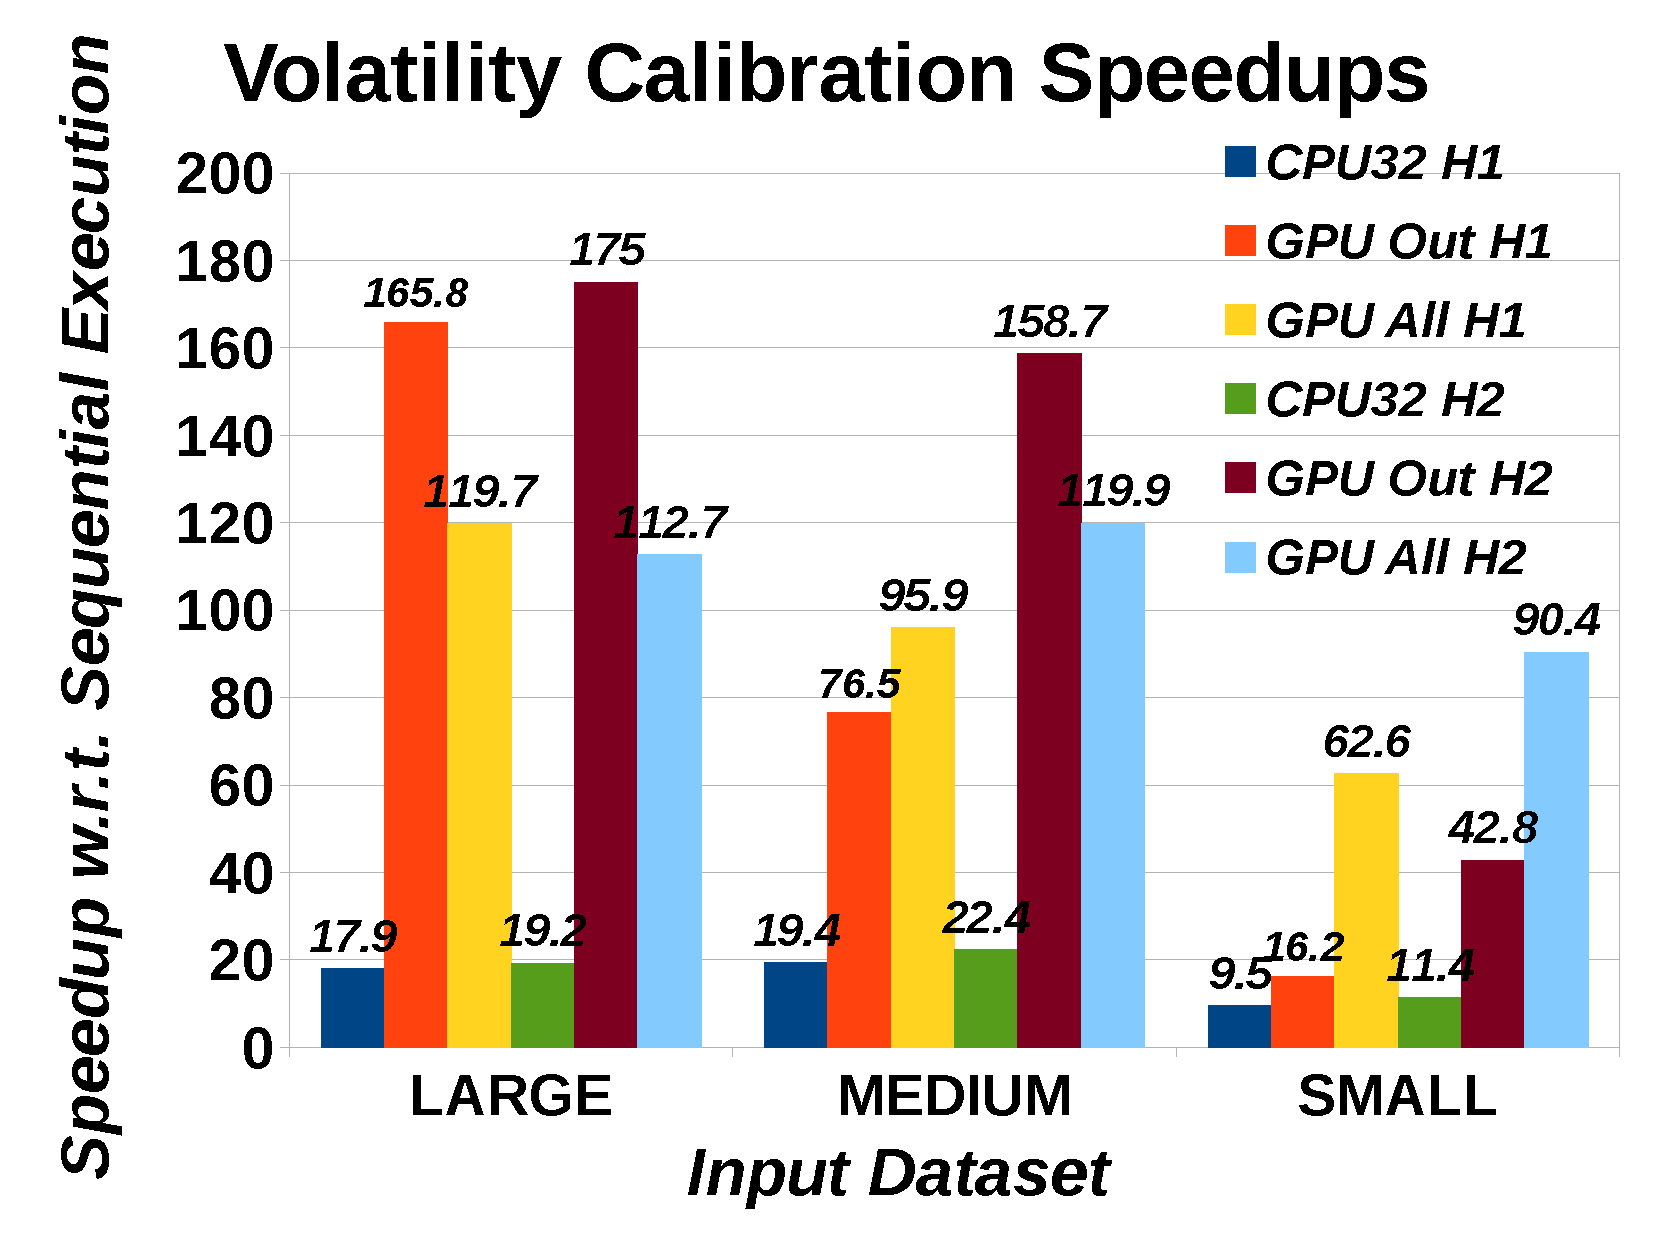
\includegraphics[height=37ex]{Figures/VolCalibRes} 
\end{center} 

%Code resemables not at all the original.

\end{frame}

\subsection{Interest-Rate Calibration}

\begin{frame}[fragile,t]
    \frametitle{Interest-Rate Calibration}

A dynamic evolution model method, i.e., genetic algorithm,
for calibrating the interest rate based on a known history
of swaption prices.\bigskip

Briefly, the interest rate is modelled as a sum of two stochastic 
processes, which gives four unknown (real) parameters, and in 
addition the two processes are assumed correlated as well, 
i.e., a fifth parameter.\bigskip

These five (unknown) parameters appear in the formula that 
computes the swaption's price, i.e., numerical integration
via hermitian-polynomials approximation.\bigskip

The genetic algorithm is used to find the five parameters 
that best fit the (known) history of swaption prices.

\end{frame}


\begin{frame}[fragile,t]
    \frametitle{Interest Rate Calibration Results}

Irregular parallelism, e.g., inner array, which is reduced, of size: $2 - 64$.
%
Not very optimized. Room for improvement.\smallskip

H1 Sequential: 510 seconds. H2 Sequential: 660 seconds.

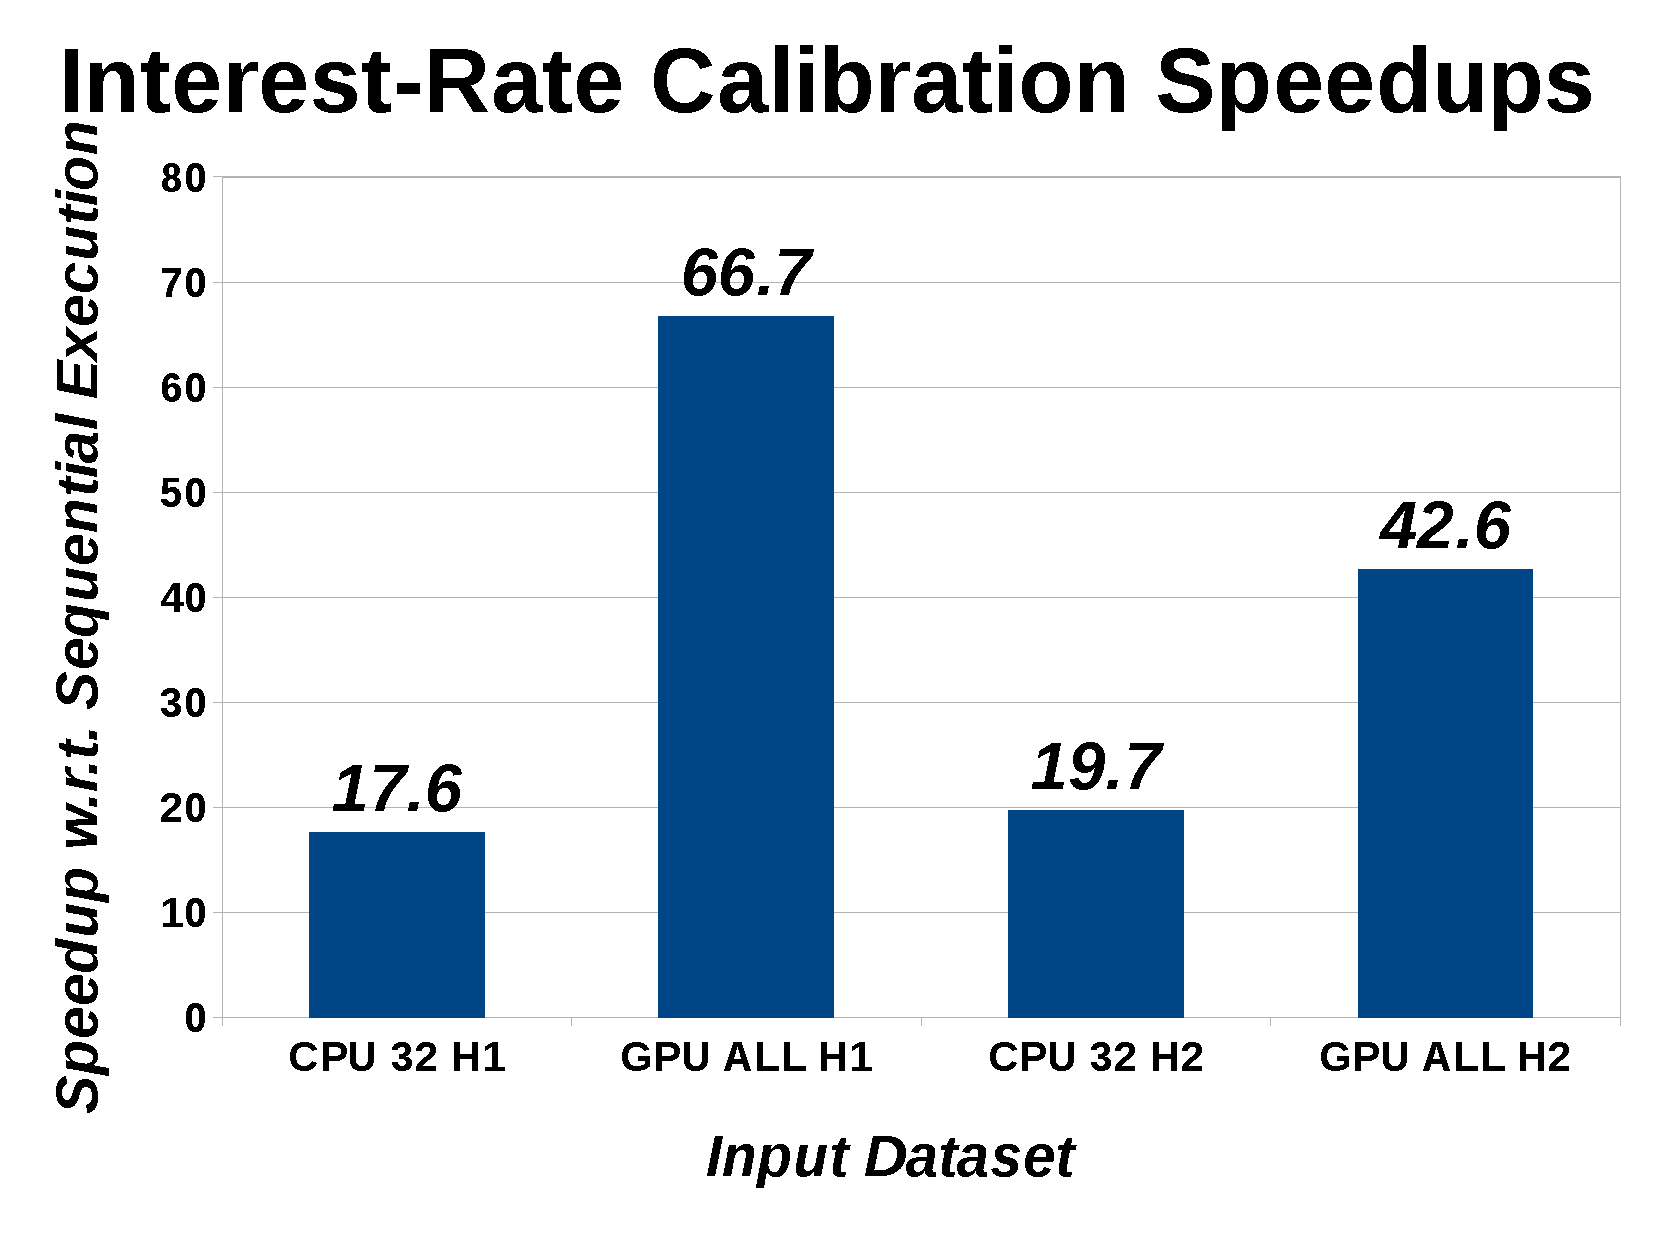
\includegraphics[width=0.80\textwidth]{Figures/InterestRateCalibRes.pdf} 

\end{frame}

\subsection{Engineering a Solution}

\begin{frame}[fragile,t]
  \frametitle{What Is The Plan?}

\begin{itemize}
    \item good expressiveness $\Rightarrow$ \emp{nested}, 
                bulk parallelism on regular arrays,\smallskip
    \item high-order invariants, e.g., \emp{map fusion}, 
                $\Rightarrow$ \emp{pure functional}\smallskip
    \item One size does NOT fit all $\Rightarrow$ \emp{``incremental flattening''}:
            \begin{itemize} 
                \item cascade of code versions,
                \item each optimized for a class of datasets,
                \item discriminated by an ``inspector'' predicate (slicing).
                \item full flattening as a baseline if everything else fails.
                \item \blue{similarities with imperative-parallelization approach}.
            \end{itemize}\smallskip

    \item transition towards an imperative rep $\Rightarrow$
                \emp{loop, in-place update},
    \item locality of reference $\Rightarrow$ \emp{imperative optimizations}, 
                    e.g., loop interchange, tiling.\medskip

    \item Challange: recovering efficient memory usage.

\end{itemize}

\smallskip

\tiny{C.~Oancea et. al., ``Financial software on GPUs: between Haskell and Fortran'', FHPC'12.\\
T.~Henriksen and C.~Oancea, ``A T2 Graph-Reduction Approach To Fusion'', FHPC'13.\\
T.~Henriksen, M.~Elsman and C.~Oancea. ``Size Slicing - A Hybrid Approach to Size Inference in Futhark'', FHPC'14.\\
T.~Henriksen and C.~Oancea. ``Bounds Checking: An Instance of Hybrid Analysis'', Array'14.\\
C.~Oancea, et. al., ``A Financial Benchmark for GPGPU Compilation'', CPC'15.
}

\end{frame}


\end{document}
